\documentclass[a4paper,11pt]{article}

\usepackage{amsmath}
\usepackage{amssymb}
\usepackage{graphicx}
\usepackage{epstopdf}
\epstopdfsetup{update}

\newcommand{\ba}{\begin{array}}
\newcommand{\ea}{\end{array}}

\newcommand{\bea}{\begin{eqnarray}}
\newcommand{\eea}{\end{eqnarray}}

\newcommand{\bc}{\begin{center}}
\newcommand{\ec}{\end{center}}

\newcommand{\ds}{\displaystyle}

\newcommand{\bt}{\begin{tabular}}
\newcommand{\et}{\end{tabular}}

\newcommand{\bi}{\begin{itemize}}
\newcommand{\ei}{\end{itemize}}

\newcommand{\bd}{\begin{description}}
\newcommand{\ed}{\end{description}}

\newcommand{\bp}{\begin{pmatrix}}
\newcommand{\ep}{\end{pmatrix}}

\newcommand{\pd}{\partial}
\newcommand{\sech}{\mbox{sech}}

\newcommand{\cf}{{\it cf.}~}

\newcommand{\ltwo}{L_{2}(\mathbb{R}^{2})}
\newcommand{\smooth}{C^{\infty}_{0}(\mathbb{R}^{2})}

\newcommand{\br}{{\bf r}}
\newcommand{\bk}{{\bf k}}
\newcommand{\bv}{{\bf v}}

\newcommand{\gnorm}[1]{\left|\left| #1\right|\right|}
\newcommand{\ipro}[2]{\left<#1,#2 \right>}

\title{Evolution of Spectral Distributions in Deep-Water Constant Vorticity Flows}
\author{Christopher W. Curtis and Mackensie Murphy}
\date{}
\begin{document}
\maketitle
\section*{Abstract}
A central question in sea-state modeling is the role that various physical effects have on the evolution of the statistical properties of random sea states.  This becomes a critical issue when one is concerned with the likelihood of rare events such as rogue, or freak, waves which can have significant destructive potential on deep sea ships and other offshore structures.  In this paper then, using a recently derived higher-order model of deep water nonlinear waves, we examine the impact of constant vorticity currents on the statistical properties of nonlinearly evolving random sea states.  As we show, these currents can both decrease and increase the kurtosis of the affiliated distributions of the sea states, thereby diminishing or enhancing the likelihood of rare events.   We likewise numerically study the relationship between the kurtosis and a non-dimensional parameter, the Benjamin--Feir Index, which has proven to be a useful measure of when rare events are likely in oceanographic application.  

\section{Introduction}
There is now a wide range of literature which shows that nonlinear instabilities, in particular the modulational instability (MI), are responsible for significant modifications to the statistical properties of water waves; see \cite{dysthe2,dysthe3,onorato,thomas2012nonlinear} among others.   As explained in \cite{janssen}, MI is especially important due to the relative rapidity with which it acts, being orders of magnitude faster than say four-wave resonant interactions which form the traditional backbone of our understanding of how nonlinearity drives changes in statistics of random-wave fields \cite{hasselmann,holthuijsen}.  These results have significant impact on the understanding of deep-water-rogue wave formation among other oceanographic phenomena.  

However, much of the understanding around MI relies on highly idealized assumptions which cannot be expected to hold in natural settings.  In particular, most understandings of MI rely on looking at the stability of perturbations to carrier waves at essentially a fixed wave number.  To address this shortcoming, in now seminal papers, \cite{alber} and \cite{alber2} analytically studied families of perturbations of wave packets with narrow, but non-zero, spectral width around a central wave number.  Using the Nonlinear Schr\"{o}dinger equation (NLSE), an analytic criterion determining when MI is either manifested or suppressed depending on this spectral width, now referred to as a Benjamin--Feir index (BFI) was derived.  The results in \cite{alber} were explored numerically in \cite{dysthe2,dysthe3} by examining the mean properties associated with ensembles of initial conditions.  

As shown in \cite{janssen} though, the movement of eigenvalues and corresponding bifurcation in stability predicted in \cite{alber} appears at best in an ambiguous fashion.  Regardless though, the BFI was still shown in \cite{janssen} to be an especially useful parameter since it allows for a ready prediction of the kurtosis of a random wave field as a quadratic function of the BFI.  Thus, the BFI becomes a useful predictive tool for the appearance of rare events, such as rogue waves in a random-nonlinear-wave field.  Experimental explorations of the results in \cite{janssen} and \cite{alber} were undertaken in \cite{onorato}, where the role of using higher-order nonlinear models than the NLSE were examined as well.  

Later work has simulated the impact of wind and damping on the interplay between the BFI and the kurtosis of a wave field; see \cite{slunyaev,eeltink}.  However, the impact of vorticity was not taken into account in these works, thereby ignoring a central mechanism for the transfer of energy across length scales in oceanic flows.  Moreover, as shown recently in \cite{curtis8}, linear shear profiles can have strong impacts on the behavior of mean properties of surface wave flows with some shear profiles being able to suppress the Stokes Drift at the surface.  Therefore while a relatively idealized case of shear, the interplay between nonlinearity and constant vorticity can manifest in markedly different physics.  Building then on the work in \cite{thomas2012nonlinear} and \cite{curtis8}, and complementing the results in \cite{touboul}, we numerically explore the statistical properties of random-nonlinear-wave fields moving over deep water and linear shear profiles.  Moving beyond just examining the properties of the NLSE with vorticity, we look at the statistical properties of solutions to a higher-order model, the vor-Dysthe equation (VDE) derived in \cite{curtis8}.  As shown in \cite{onorato,janssen} and \cite{eeltink}, the higher-order terms associated with the Dysthe equation can have significant impacts on the statistics of the waves, so it is a nontrivial question to examine how the vorticity interacts with these higher-order nonlinearities.  

Using our simulations, starting from normally distributed random-wave fields, we show that the BFI condition with respect to predicting stability is not especially useful, conforming to the results in \cite{janssen}.  While we are able to show that for sufficiently wide enough initial distributions that the temporal modifications to the profile are slight, whether or not this corresponds to an actual bifurcation in stability or simply reflects that for a wide enough profile the sideband growth affiliated with the MI has little impact is not clear.  We note though that classic MI analysis does provide a useful prediction of the time scale over which the most significant dynamics in the statistics of the wave field occur.  

Beyond the issue of MI, we see several interesting results from our work.  In particular, we see that increasing vorticity enhances the kurtosis of the random-wave field.  Moreover, the VDE always predicts a larger kurtosis than the NLSE, with this difference between the models exacerbated by increasing vorticity.  Likewise the affiliated statistics of the spectral distribution show marked differences between the two models, with the VDE tending to strongly skew distributions away from Gaussian conditions through peak down shifting and one sided tail enhancement.  Finally, we study the behavior of the kurtosis as a function of the BFI parameter.  The quadratic relationship found in \cite{janssen} and \cite{eeltink} is shown to hold, though the nature of the fit is clearly dependent on the vorticity, conforming to the dependence of the fit on physical parameters found in \cite{eeltink}.

 Thus we show that vorticity and higher-order deep water models can have significant impacts on our understanding of the likelihood of rare events, like rogue waves, in deep-water-surface flows.  In particular, shear profiles which tend to propagate in the direction of the surface wave-field acting on relatively narrow distributions of waves can create strongly non-Gaussian distributions with significantly enhanced tails thereby encouraging the occurrence of rare events.  These results motivate further study of currents in random-wave fields, especially as they pertain to the presence of wind and wave dissipation.  

The structure of the paper is an explanation of the model and discussion of the BFI in Section 2.  Section 3 presents our numerical results, while Section 4 presents a conclusion.  

\section{Modeling and Stability Theory}
We examine the unsteady nonlinear wave propagation over a constant shear current.  To do this, we suppose the fluid velocity is of the form
\[
{\bf u} = u({\bf x},t)\hat{{\bf x}} + w({\bf x},t)\hat{{\bf z}} = \omega z\hat{{\bf x}} + \nabla \phi,
\]
where $\phi$ is a harmonic function.  We restrict fluid motion to the $(x,z)$-plane, thereby ignoring transverse variations in the $y$ dimension.   Using well established arguments, e.g.~see \cite{ashton}, the dynamics of the fluid are found by solving the free boundary value problem
\begin{align}
\Delta \phi = 0, & & -\infty< z < \eta(x,t), \nonumber \\
\eta_{t} +\left(\omega\eta+\phi_{x}\right)\eta_{x} - \phi_{z} = 0, & & z=\eta(x,t), \label{kine}\\
\phi_{t} + \omega\pd_{x}^{-1}\eta_{t} + \frac{1}{2} \left|{\bf
    u}\right|^{2} + g\eta -
\frac{\sigma}{\rho}\pd_{x}\frac{\eta_{x}}{\sqrt{1+\eta_{x}^{2}}}= 0, &
& z=\eta(x,t), \label{bernou}\\
\lim_{z\rightarrow -\infty} \phi_{z} = 0, \nonumber
\end{align}
where $\eta$ represents the free surface displacement, and $g$, $\rho$, and $\sigma$ represent the acceleration due to gravity, the fluid density, and the coefficient of surface tension respectively.  The system is non-dimensionalized via the choices 
\begin{align*}
\tilde{x} = \frac{x}{L_{p}}, ~\tilde{z} = \frac{z}{L_{p}}, ~ \tilde{t} = \sqrt{\frac{g}{L_{p}}}~t, ~\omega = \sqrt{\frac{g}{L_{p}}}~\tilde{\omega}, \\
\eta = a \tilde{\eta}, ~ \phi  = a\sqrt{gL_{p}}~\tilde{\phi} , ~ \epsilon = \frac{a}{L_{p}}.
\end{align*}
Note that we are assuming $\omega = \mathcal{O}(1)$ throughout the remainder of the paper.  In physical terms, this implies that $\omega$ is comparable to the natural time scale of this problem, $\sqrt{L_{p}/g}$.  If we were to assume $\omega$ were of larger magnitude, the problem would no longer be weakly nonlinear and asymptotic analysis would be siginificantly more difficult.  Therefore, throughout the remainder of the paper, we assume that the vorticity is not too large.

For a relatively small free-fluid surface over infinitely-deep water $z=\epsilon \eta(x,t)$, we model a modulated-wave packet via the expansion 
\begin{multline*}
\eta(x,t) = \eta_{1}(\xi,\tau)e^{i\theta(x,t)} + \eta^{\ast}_{1}(\xi,\tau)e^{-i\theta(x,t)}\\
+ \epsilon\left(\eta_{0}(\xi,\tau) + \eta_{2}(\xi,\tau)e^{2i\theta(x,t)} + \eta^{\ast}_{2}(\xi,\tau)e^{-2i\theta(x,t)}\right) + \mathcal{O}\left(\epsilon^{2} \right)
\end{multline*}
where $\tau = \epsilon^{2}t$, $\xi = \epsilon(x+c_{g}t)$, and $\theta(x,t) = k_{0}x + \Omega(k_{0},\omega)t$, where the linear dispersion relationship $\Omega(k_{0},\omega)$ is given by
\[
\Omega(k_{0},\omega) = \frac{1}{2}\left(s\omega \pm \sqrt{\omega^{2} + 4|k_{0}|\left(1+\tilde{\sigma}k_{0}^{2}\right)} \right).
\]
We note that the form for $\phi$ follows directly from this expansion, allowing for everything to be modeled by the terms in the expansion in $\eta$.  Here, $s = \mbox{sgn}(k_{0})$, $\omega$ is the non-dimensionalized magnitude of the vorticity of the flow, and $\tilde{\sigma}$ is the surface tension, or where the reciprocal of the Bond number, $\tilde{\sigma}$, is given by
\[
\tilde{\sigma} = \frac{\sigma}{\rho g L_{p}^2}.
\]
Throughout the remainder of this paper, we take the positive branch $+$ of the dispersion relationship, thereby ensuring that $\Omega > 0$.  Thus, for $k_{0}>0$, the surface waves to leading order propagate to the left.  Thus, if $\omega>0$, then throughout the bulk of the fluid, the shear current propagates with the surface waves, or is {\it co-propagating}, while for $\omega<0$, we say the shear current is {\it counter-propagating}.  

To describe the evolution of the slowly evolving envelope $\eta_{1}(\xi,\tau)$, we use two models.  The first model is the the nonlinear Schr\"{o}dinger equation (NLSE) derived in \cite{curtis8}, though see also \cite{thomas2012nonlinear}, given by 
\[
i\pd_{\tau}\eta_{1} + \alpha_{d}\pd_{\xi}^{2}\eta_{1} + \alpha_{nl}\left|\eta_{1} \right|^{2}\eta_{1} = 0, 
\]
where 
\begin{align*}
c_{g} = & \frac{1+3\tilde{\sigma}k_{0}^{2}}{2s\Omega - \omega},\\
\alpha_{d}(k_{0},\omega) = & \frac{(c^2_{g} - 3|k_{0}|\tilde{\sigma})}{2\Omega-s\omega},\\
\alpha_{nl}(k_{0},\omega) = & \frac{k_{0}\left( sk_{0}^{3}\left(8 + \tilde{\sigma}k_{0}^{2} + 2(\tilde{\sigma}k_{0}^{2})^{2}\right) + \omega \alpha_{v}\right)}{\left(2s\Omega -\omega\right)(1+c_{g}\omega)\left(4\Omega^2-s(2k_{0}(1+4\tilde{\sigma}k_{0}^{2})+2\omega\Omega)\right)}.
\end{align*}
However, the NLSE is a relatively low-order model known to be only of limited use in real-world modeling situations.  A more robust model, following the work in \cite{dysthe1}, is found by going to the next higher order in $\epsilon$, giving us the equation
\begin{multline}
(\omega-2s\Omega)\pd_{\tau}\eta_{1} + i(c_{g}^{2}s-3k_{0}\tilde{\sigma})\pd_{\xi}^{2}\eta_{1} + 2i\epsilon s c_{g}\pd^{2}_{\xi\tau}\eta_{1} - \epsilon\tilde{\sigma} \pd^{3}_{\xi}\eta_{1} + i\epsilon^{2}c_{h}\pd_{\xi}^{4}\eta_{1} \\
- i \alpha_{nl}(\omega-2s\Omega)\left|\eta_{1}\right|^{2}\eta_{1}
+ \epsilon \tilde{\alpha}_{1}\left|\eta_{1}\right|^{2}\pd_{\xi}\eta_{1}\\
+ \epsilon\tilde{\alpha}_{2}\eta_{1}^{2}\pd_{\xi}\eta^{\ast}_{1} +
\epsilon i\tilde{\alpha}_{3}\eta_{1}\mathcal{H}\pd_{\xi}\left|\eta_{1}\right|^{2}= 0.
\label{dysthe}
\end{multline}
where $\mathcal{H}$ denotes the Hilbert transform so that 
\[
\mathcal{H}f = \frac{1}{2\pi}\int_{\mathbb{R}}dk~ e^{ikx}  i\mbox{sgn}(k) \hat{f}(k),
\]
and where $\hat{f}(k)$ is the Fourier transform of $f(x)$ defined by
\[
\hat{f}(k) = \int_{\mathbb{R}}dx~ e^{-ikx}f(x).
\]

We call Equation \eqref{dysthe} the Vor-Dysthe equation (VDE).  Details of its derivation can be found in \cite{curtis8}, though we note a difference in this work with that in \cite{curtis8}.  In this work, we found the inclusion of the higher-order dispersion associated with the coefficient $c_{h}$, given by
\[
c_{h} = 2sc_{g}(2sc_{g}\alpha_{d}+\tilde{\sigma})/(\omega-2s\Omega) - s\alpha_{d}^{2},
\]
was necessary to remove artificial numerical instabilities.  Similar issues with Dysthe like equations have been noted in \cite{eeltink} among other sources.  Moreover, the coefficients $\tilde{\alpha}_{j}$ are readily derived, but their forms are cumbersome and thus we omit explicitly writing them for the sake of readability.  

To generate simulations, we start both the NLSE and VDE from the same collection of $2L$ periodic-initial conditions
\[
\eta_{1}(\xi,0) = \epsilon_{rms}\sqrt{\frac{\delta \tilde{k}}{\sigma\sqrt{\pi}}} \sum_{k=-K+1}^{K}e^{-\tilde{k}^{2}/2\sigma^{2}}e^{i\theta_{k}}e^{i\tilde{k}\xi}, ~ \tilde{k} = \frac{\pi k}{L},
\]
where $\delta \tilde{k}=\pi/L$ and the phases $\theta_{k}$ are randomly and independently chosen uniformly between $0$ and $2\pi$.  We can then readily show that, for $L\gg 1$, 
\[
\epsilon_{rms} \approx \overline{\left|\eta_{1}(\xi,0)\right|^{2}}^{1/2},
\]
where $\overline{()}$ denotes the ensemble average.  In our coordinates then, motivated by the work of \cite{alber} and \cite{dysthe2} and more fully explored in \cite{janssen}, we study the stability of the initial wavepacket distributions with regards to the magnitude of the Benjamin--Feir Index (BFI), where the BFI is defined to be  
\[
\mbox{BFI} = \sqrt{\frac{\alpha_{nl}}{\alpha_{d}}}\frac{\epsilon_{rms}}{\sigma}.
\]
Note, this definition is identical with the spectral width criterion of \cite{alber} and the BFI condition given in \cite{thomas2012nonlinear}; see also \cite{onorato}.  It was claimed in \cite{alber}, and in some sense verified in \cite{dysthe2}, that wave packets should be stable with respect to MI's for $\mbox{BFI}<1$, which corresponds to the initial spectral width $\sigma>\sigma_{c}$, where 
\[
\sigma_{c} = \sqrt{\frac{\alpha_{nl}}{\alpha_{d}}}\epsilon_{rms}.
\]

However, \cite{alber} does not present numerical verification of their results, and \cite{dysthe2} is relatively brief in their verification of the BFI condition.  The work in \cite{janssen} shows that the BFI condition does not yield a clear bifurcation in stability.  Our results likewise support this.  However, also shown in \cite{janssen} and followed up on in several later works; see \cite{onorato,slunyaev,eeltink}, it is shown that the kurtosis of the corresponding distribution of the surface waves, say $\tilde{k}(\tau)$ is a quadratic function of the time evolving $\mbox{BFI}(\tau)$.   We likewise aim to establish a similar relationship, thereby maintaining the utility of the BFI insofar as it then helps predict a key feature of nonlinear-random wave fields. 
%%%%%%%%%%%%%%%%%%%%%%%%%%%%%%%%%%%%%%%%%%%%%%%%%%%%%%%%%%%%%%%%%%%%%%%%%%%%%%%%%%%
%%%%%%%%%%%%%%%%%%%%%%%%%%%%%%%%%%%%%%%%%%%%%%%%%%%%%%%%%%%%%%%%%%%%%%%%%%%%%%%%%%%
\section{Results}
To understand the relationship between the vorticity $\omega$ and the initial spectral width $\sigma$ of our initial conditions, we generate ensembles of initial conditions and then run these different initial conditions up to $\tau_{f}$ where $\tau_{f}$ is given by
\[
\tau_{f}=\max\left\{1.5/\alpha_{nl},1\right\},
\]
so that MI has a sufficiently long enough time scale over which to act; see \cite{curtis8} for a derivation of this result.  We choose $L=5\pi$ so that the computational domain is $[-5\pi,5\pi]$.  The number of modes is $K_{T} = 1024$ or $K=512$.  The surface tension is $\tilde{\sigma} = 10^{-5}$. We then compute the averaged spectral density $S(k,\tau;\sigma)$ where 
\[
S\left(k,\tau;\sigma\right) \sim \overline{\left( \left|\hat{\eta}_{1}\left(k,\tau;\sigma \right)\right|^{2}\right)},
\]
which corresponds to the autocorrelation of the surface profile with respect to space.  Note, we normalize $S$ so that it is a probability distribution.  Using $S(k,\tau_{f},\sigma)$, we then plot the time dynamics of the mean $m(\tau)$
\[
m(\tau) = \int_{\mathbb{R}} k S\left(k,\tau;\sigma\right) dk,
\]
standard deviation $\tilde{\sigma}(\tau)$,
\[
\tilde{\sigma}(\tau) = \left(\int_{\mathbb{R}} (k-m(\tau))^{2} S\left(k,\tau;\sigma\right) dk\right)^{1/2},
\]
and the kurtosis $\tilde{k}(\tau)$
\[
\tilde{k}(\tau) = \frac{1}{3\tilde{\sigma}^{4}(\tau)}\int_{\mathbb{R}} (k-m(\tau))^{4} S\left(k,\tau;\sigma\right) dk - 1,
\]
so as to examine the impact of various shear profiles on the statistics of the waves as well as establishing that statistical equilibrium has been achieved by $\tau_{f}$.  Note, we interpret the kurtosis $\tilde{k}$ as the degree to which the distribution $S$ exhibits `heavy-tail phenomena', or the enhancement of the probability of what should otherwise be rare events.  Given that all Gaussian distributions have $\tilde{k}=0$, all measurements are then made relative to this fixed level.  Moreover, following the approach in \cite{dysthe2,dysthe3}, by comparing the initial spectral density to that at later times, we can see directly whether MI manifests as significant distortions of the statistics, or if through suppression the distributions remain relatively close to one another.  

Throughout our results, we have used a pseudo-spectral method in space coupled with a 4th-order Runge-Kutta scheme using integrating factors in time, with a time step of $dt = 1 \times 10^{-3}$.  De-aliasing is implemented via Orszag's `2/3-rule'.  Averaging was done with $N_{e}=512$ ensemble members, thereby ensuring relative averaging errors on the order of about $1\%$.  We set $\epsilon=.05$ throughout the remainder of the paper.  

\subsection*{Vorticity-Free Flow: $\omega = 0$}

We first examine the vorticity free case so as to establish a base line against which to measure non-zero shear.  Looking at the time dynamics of the affiliated statistics when the initial width $\sigma=1.05\sigma_{c}$ where $\sigma_{c}\approx 4$, we see in Figure \ref{fig:stbleom0} the final steady distribution $S$ for $\tau_{f}=1$ as well as the affiliated time dynamics of the three primary moments $m(\tau)$, $\tilde{\sigma}(\tau)$, and $\tilde{k}(\tau)$.  As can be seen, any claim of stability of the distribution for either the NLSE or VDE is tenuous at best.  Note, the timescale for MI is $1/\alpha_{nl} = .5$ in this case.  We see this result borne out in the plots in Figures \ref{fig:stbleom0} (b)-(d), which shows that saturation of the affiliated statistics does not set in till somewhat after this MI timescale.  Thus, arguing that instability with respect to MI drives the observed statistical dynamics is reasonable.  Comparing the VDE to the NLSE, we see the added nonlinearity in the VDE allows for yet greater deviations away from normality through the downshifting of the spectral peak; see Figure \ref{fig:stbleom0} (a), and the asymmetric widening of the VDE profile as evidenced by the enhanced kurtosis and strong shift in the mean as seen in Figures \ref{fig:stbleom0} (d) and (b) respectively.  

In contrast, by more than doubling the initial spectral width to $\sigma = 2\sqrt{2}\sigma_{c}$, we see in Figure \ref{fig:stbleom0wide} that an argument for stability against MI can be made.  As can be seen for both the NLSE and VDE, all of the affiliated statistics remain close to their initial values and saturate rapidly, though we again see time of onset of saturation corresponds to the MI timescale.  But as predicted in \cite{alber}, there should be profiles wide enough such that the impact of MI is nominal, though it is, as noted in \cite{janssen}, difficult to argue that what is being observed is a bifurcation as opposed to a weak nonlinear effect.   Despite the relative stability, we again note that the VDE still has significant impacts on the statistics of the spectral distribution $S$, with in particular the VDE providing a slight enhancement of the kurtosis relative to the NLSE, which essentially maintains the normality of the initial distribution.  This effect is also seen in the absence of an inversion in the magnitude of $\tilde{\sigma}(\tau)$, i.e. compare Figures \ref{fig:stbleom0} (b) to \ref{fig:stbleom0wide} (b), which shows that in the wider initial spectral width case, the VDE is wider than the NLSE, whereas in the more narrow initial spectral width case the roles between the two equations are reversed, reflecting the VDE's tendency to strongly skew $S(k,\tau_{f},\sigma)$.

\begin{figure}[!ht]
\centering
\begin{tabular}{cc}
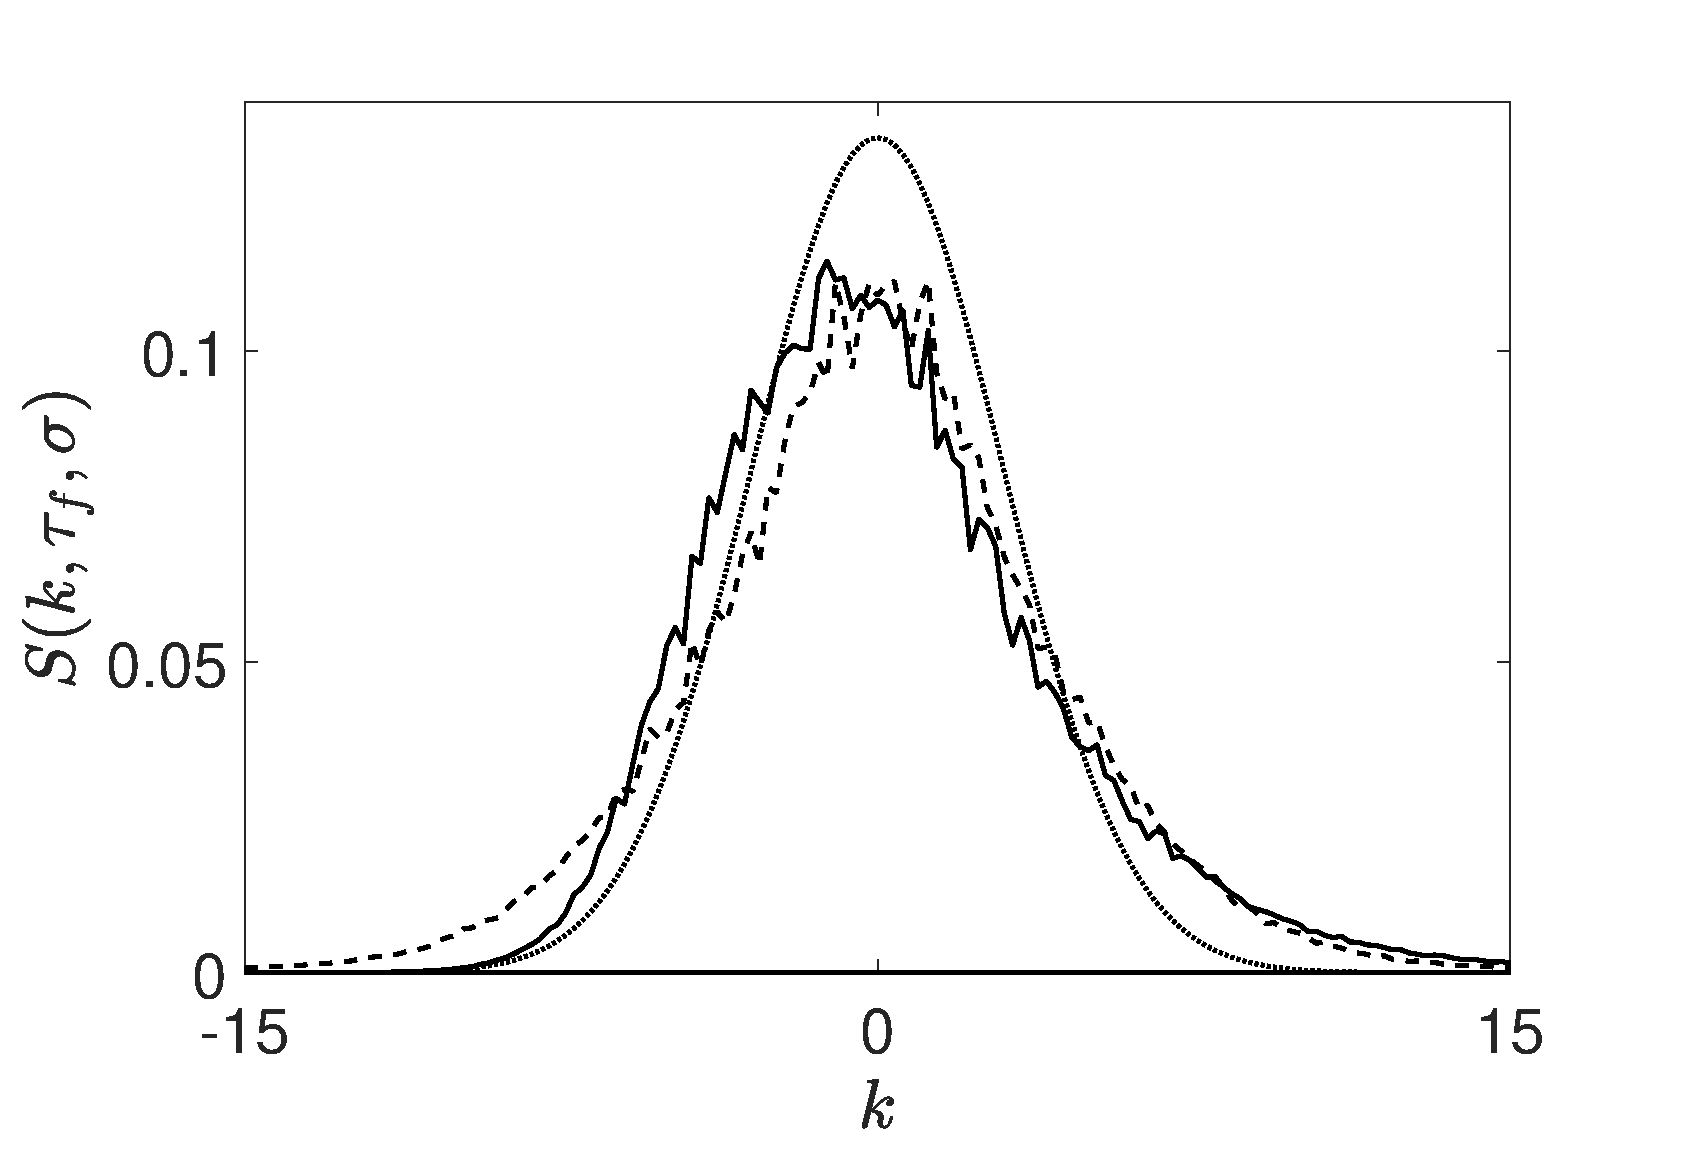
\includegraphics[width=60mm, height=39mm]{pdf_w_0_ep_pt05_Nens_512_sig0_1pt05} & 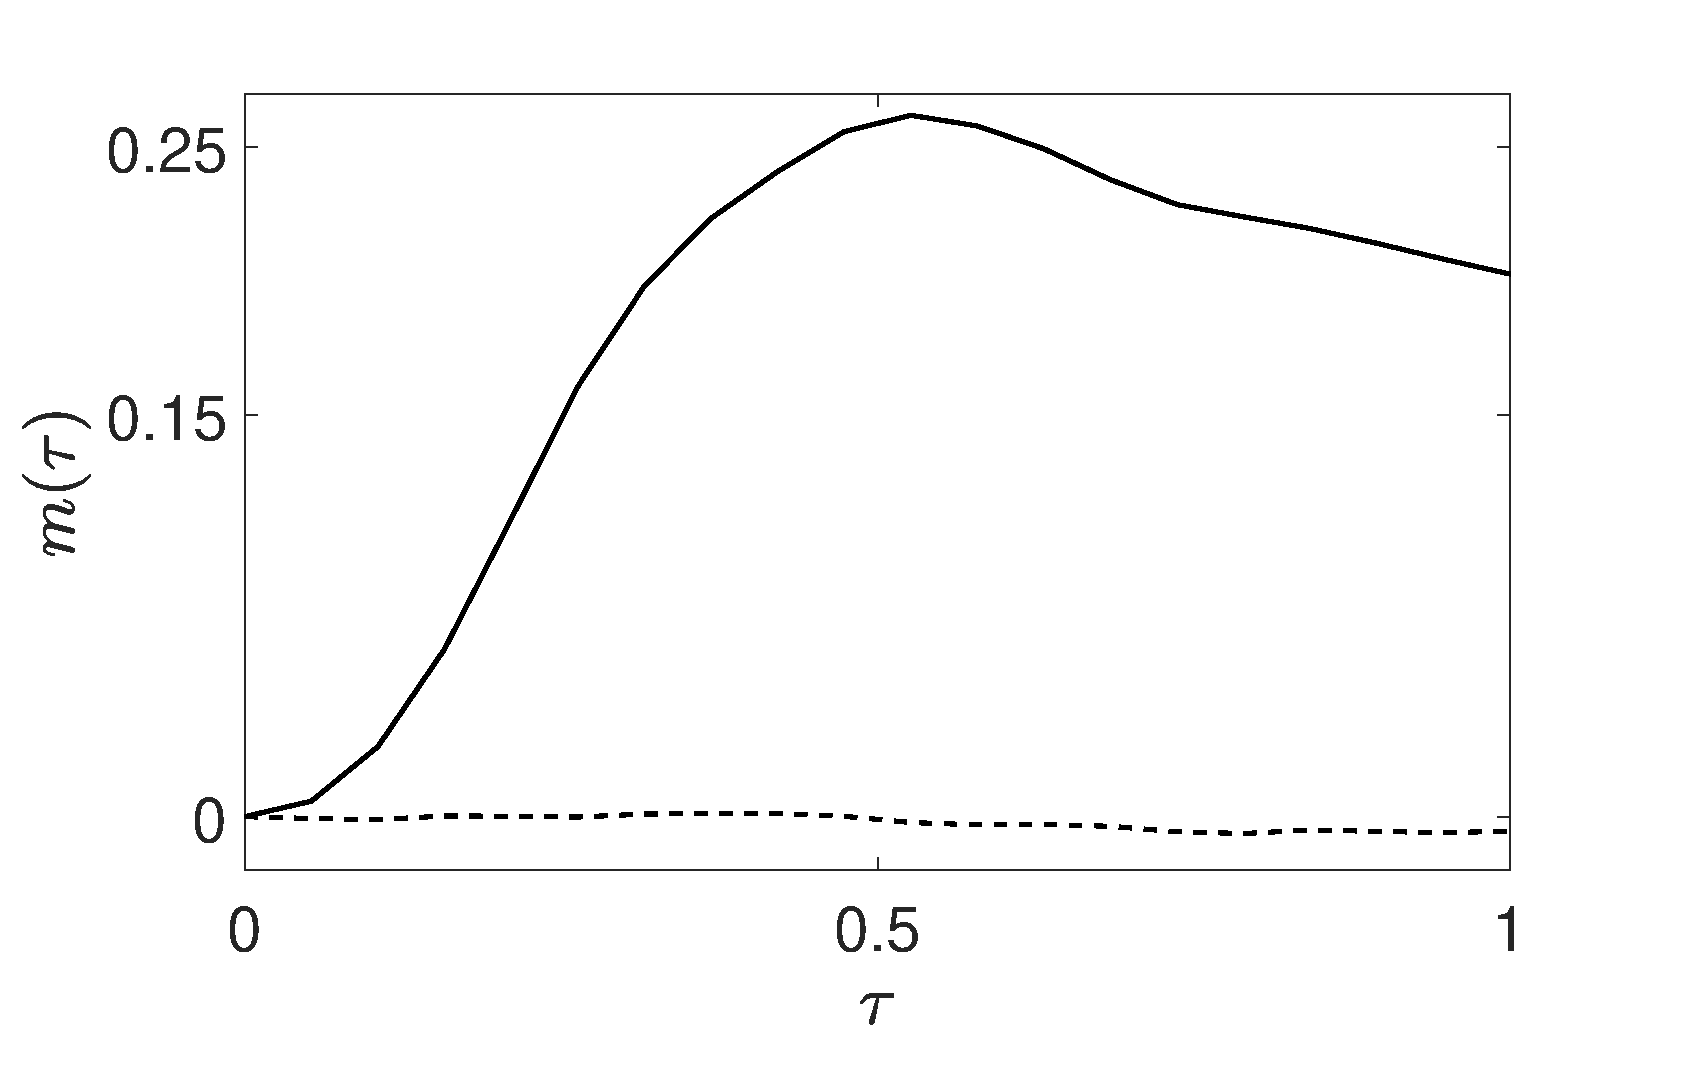
\includegraphics[width=.48\textwidth]{mean_w_0_ep_pt05_Nens_512_sig0_1pt05} \\
(a) $S(k,\tau_{f},1.05\sigma_{c})$ & (b) $m(\tau)$, $\sigma = 1.05\sigma_{c}$\\
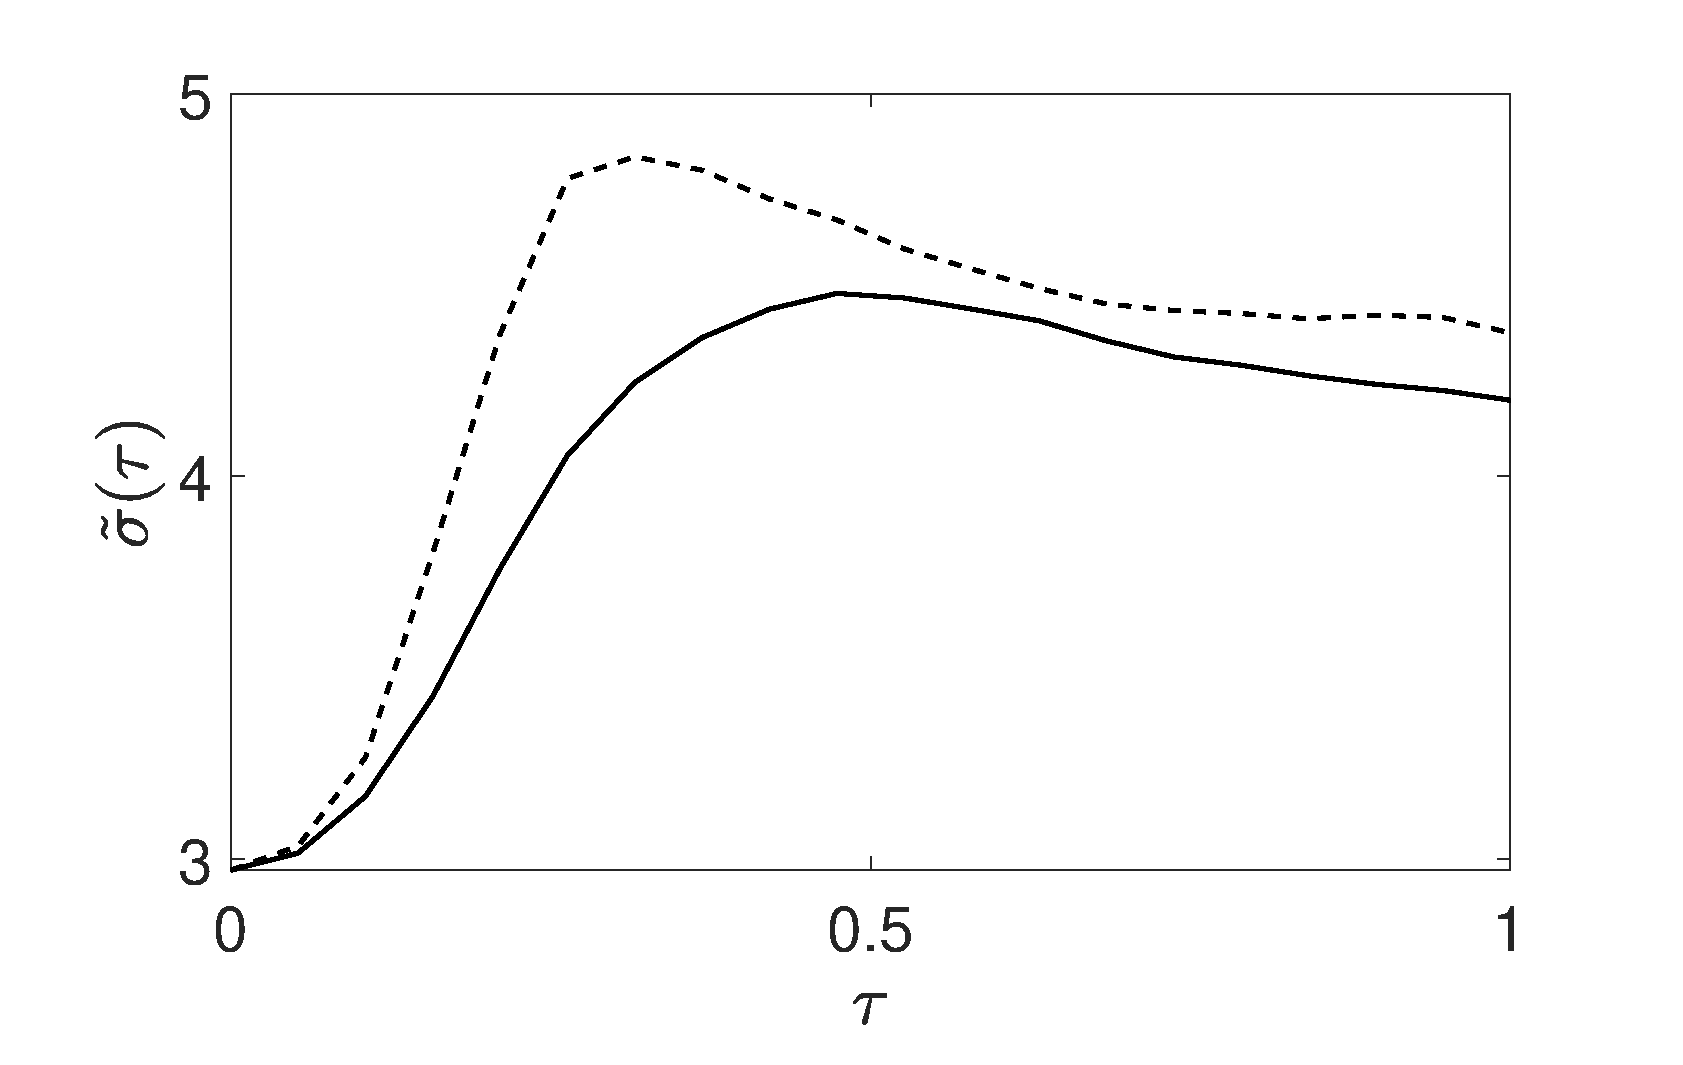
\includegraphics[width=.48\textwidth]{std_w_0_ep_pt05_Nens_512_sig0_1pt05} & \includegraphics[width=.48\textwidth]{kts_w_0_ep_pt05_Nens_512_sig0_1pt05} \\
(c) $\tilde{\sigma}(\tau)$, $\sigma = 1.05\sigma_{c}$ & (d) $\tilde{k}(\tau)$, $\sigma = 1.05\sigma_{c}$\\
\end{tabular}
\caption{For $\omega=0$ and $\sigma=1.05 \sigma_{c}$, in (a) the plot of the spectral distribution function $S(k,\tau_{f},1.05\sigma_{c})$, in (b) the plot of the mean $m(\tau)$, in (c) the plot of the standard deviation $\tilde{\sigma}(\tau)$, and in (d) the plot of the kurtosis $\tilde{k}(\tau)$.  In the graphs, the NLSE is (- -), the VDE (-), and the initial distribution is ($\cdots$).}
\label{fig:stbleom0}
\end{figure}

\begin{figure}[!ht]
\centering
\begin{tabular}{cc}
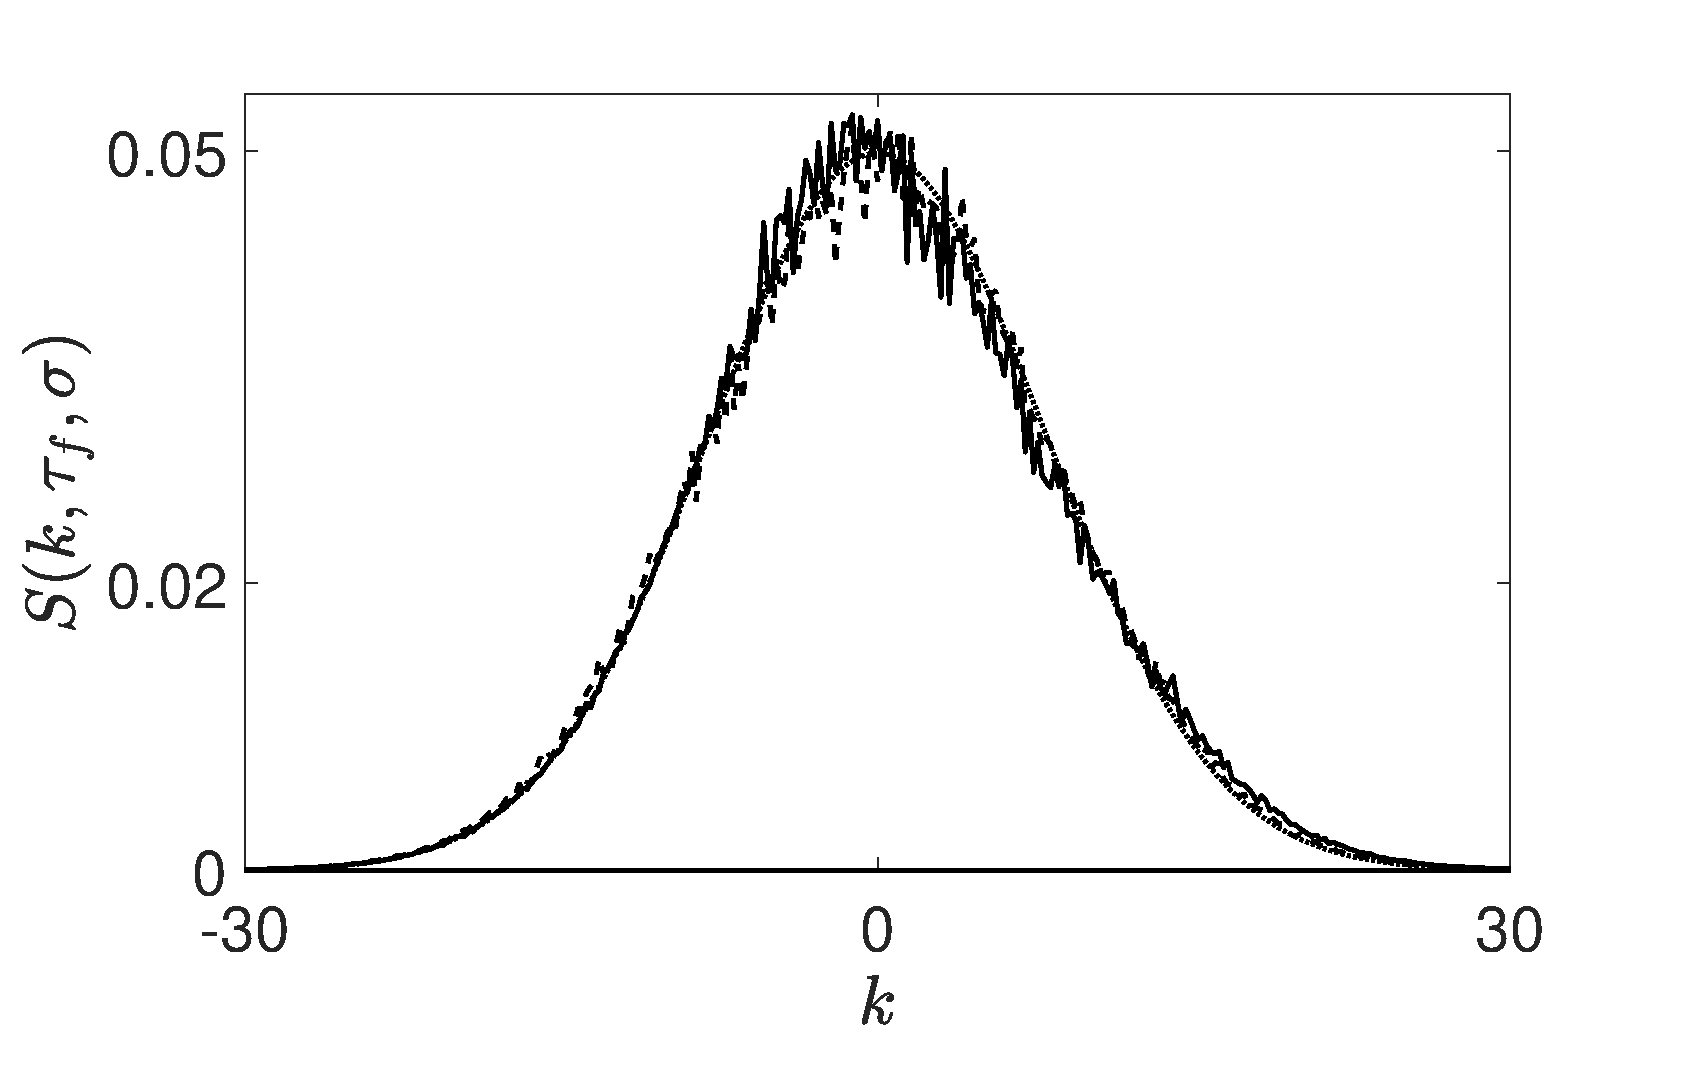
\includegraphics[width=.48\textwidth]{pdf_w_0_ep_pt05_Nens_512_sig0_2sqrt2} & \includegraphics[width=.45\textwidth]{mean_w_0_ep_pt05_Nens_512_sig0_2sqrt2} \\
(a) $S(k,\tau_{f},2\sqrt{2}\sigma_{c})$ & (b) $m(\tau)$, $\sigma = 2\sqrt{2}\sigma_{c}$\\
\includegraphics[width=.48\textwidth]{std_w_0_ep_pt05_Nens_512_sig0_2sqrt2} & \includegraphics[width=.48\textwidth]{kts_w_0_ep_pt05_Nens_512_sig0_2sqrt2} \\
(c) $\tilde{\sigma}(\tau)$, $\sigma = 2\sqrt{2}\sigma_{c}$ & (d) $\tilde{k}(\tau)$, $\sigma = 2\sqrt{2}\sigma_{c}$
\end{tabular}
\caption{For $\omega=0$ and $\sigma=2\sqrt{2} \sigma_{c}$, in (a) the plot of the spectral distribution function $S(k,\tau_{f},1.05\sigma_{c})$, in (b) the plot of the mean $m(\tau)$, in (c) the plot of the standard deviation $\tilde{\sigma}(\tau)$, and in (d) the plot of the kurtosis $\tilde{k}(\tau)$. In the graphs, the NLSE is (- -), the VDE (-), and the initial distribution is ($\cdots$).}
\label{fig:stbleom0wide}
\end{figure}

\subsection*{Counter-Propagating Shear: $\omega = -.5$}

For the first case of nontrivial shear, we look at setting $\omega=-.5$ which corresponds to the shear profile propagating against the movement of the surface wave.  This parameter choice gives us the BFI $\sigma_{c} \approx 5.5$.  Here $\tau_{f}=1$ since the MI timescale is given by $1/\alpha_{nl}\approx .3$.  As seen in Figure \ref{fig:stbleomnh}, the BFI condition does not appear to hold, with significant deviations away from the initial Gaussian profile happening on the predicted MI timescale.  Moreover, by again increasing the initial width to $\sigma = 2\sqrt{2}\sigma_{c}$, the overall impact of MI is markedly reduced, with the VDE and NLSE all but producing nearly identical results as seen in Figure \ref{fig:stbleomnhwide}.  We likewise again see the inversion in the standard deviation between the two models for the narrow initial spectral width; see Figure \ref{fig:stbleomnh} (b), while the inversion is absent in the wide initial width case; see Figure \ref{fig:stbleomnhwide}.  

That being said, while the VDE still produces a final distribution which is less Gaussian and more favorable to far tail phenomena relative to the NLSE, we also see that the counter propagating shear lowers the overall kurtosis compared to the case of $\omega=0$.   Thus while the overall distributions are wider in the $\omega=-.5$ case relative to the $\omega=0$ case, the drop in kurtosis induced by the counter-propagating shear would seem to still reduce the relative importance of far-tail phenomena.  We can then make a prediction that counter-propagating shear would generally reduce the chances of events like rogue-waves forming.  

\begin{figure}[!ht]
\centering
\begin{tabular}{cc}
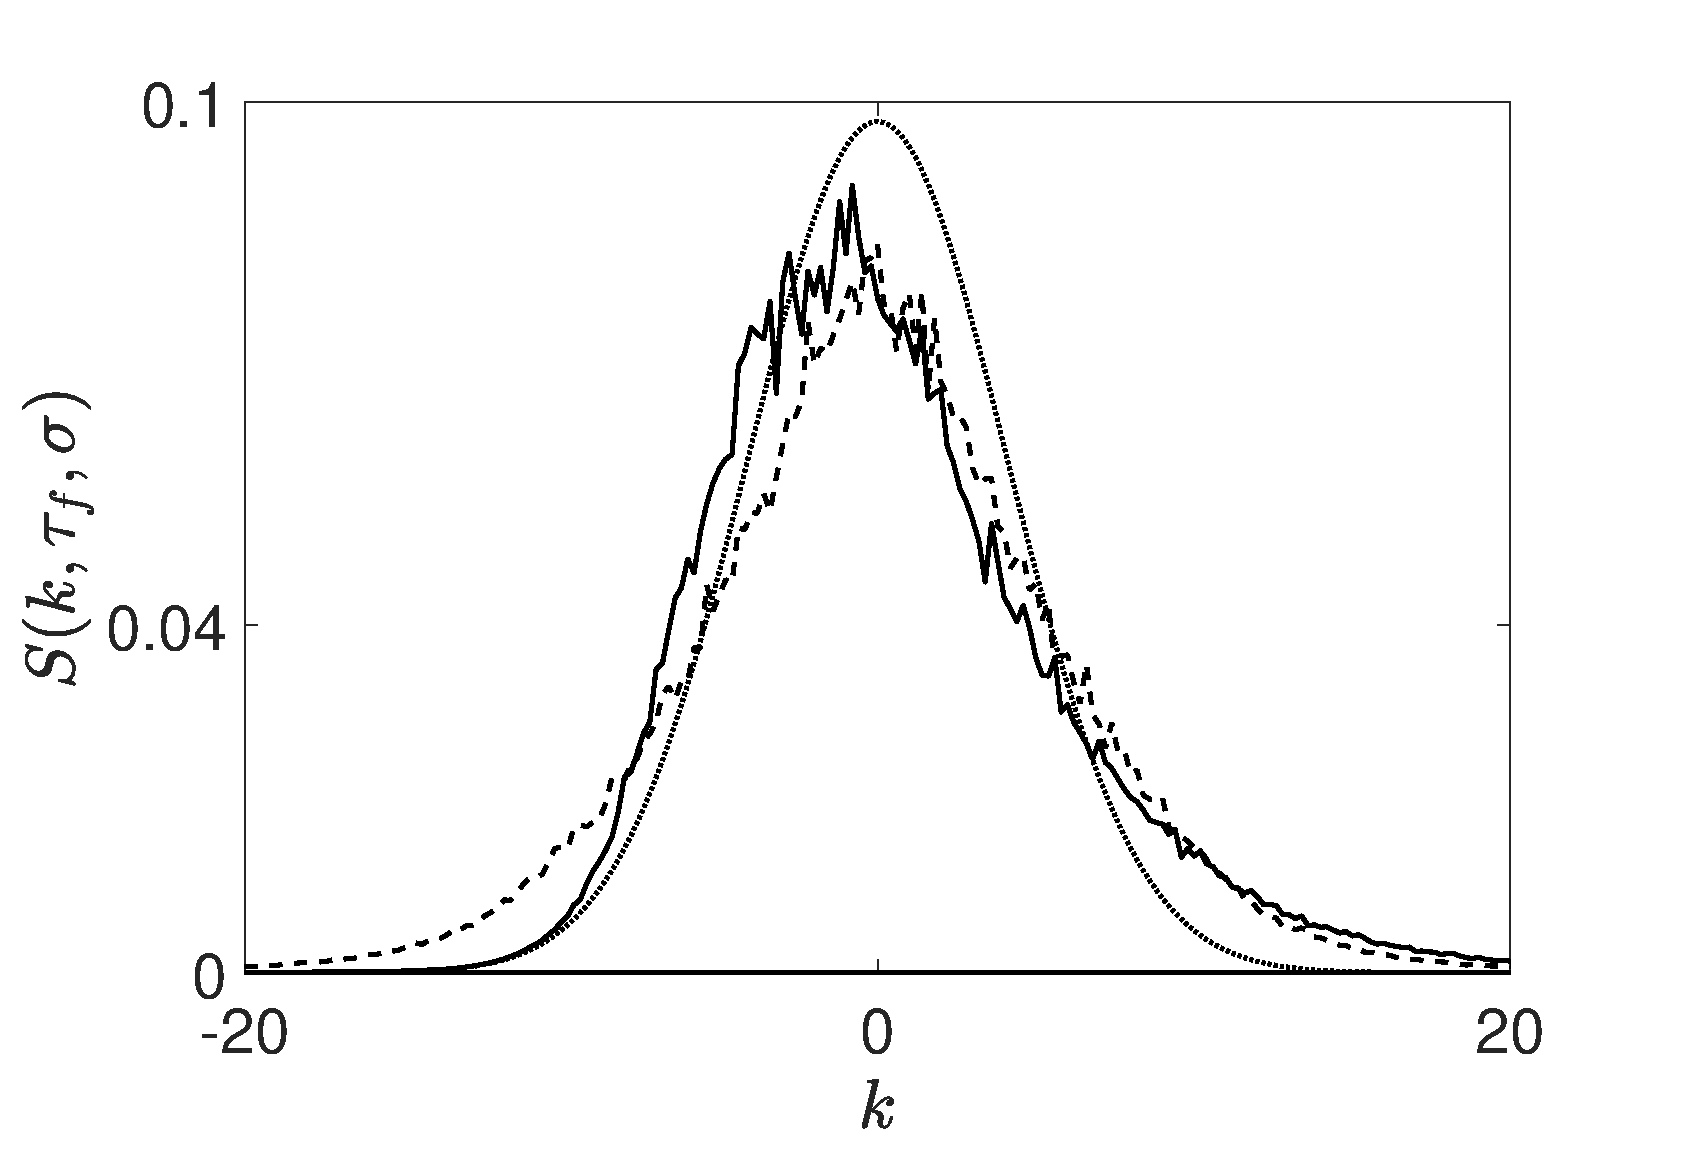
\includegraphics[width=60mm, height=39mm]{pdf_w_nhf_ep_pt05_Nens_512_sig0_1pt05} & \includegraphics[width=.48\textwidth]{mean_w_nhf_ep_pt05_Nens_512_sig0_1pt05} \\
(a) $S(k,\tau_{f},1.05\sigma_{c})$ & (b) $m(\tau)$, $\sigma = 1.05\sigma_{c}$\\
\includegraphics[width=.48\textwidth]{std_w_nhf_ep_pt05_Nens_512_sig0_1pt05} & 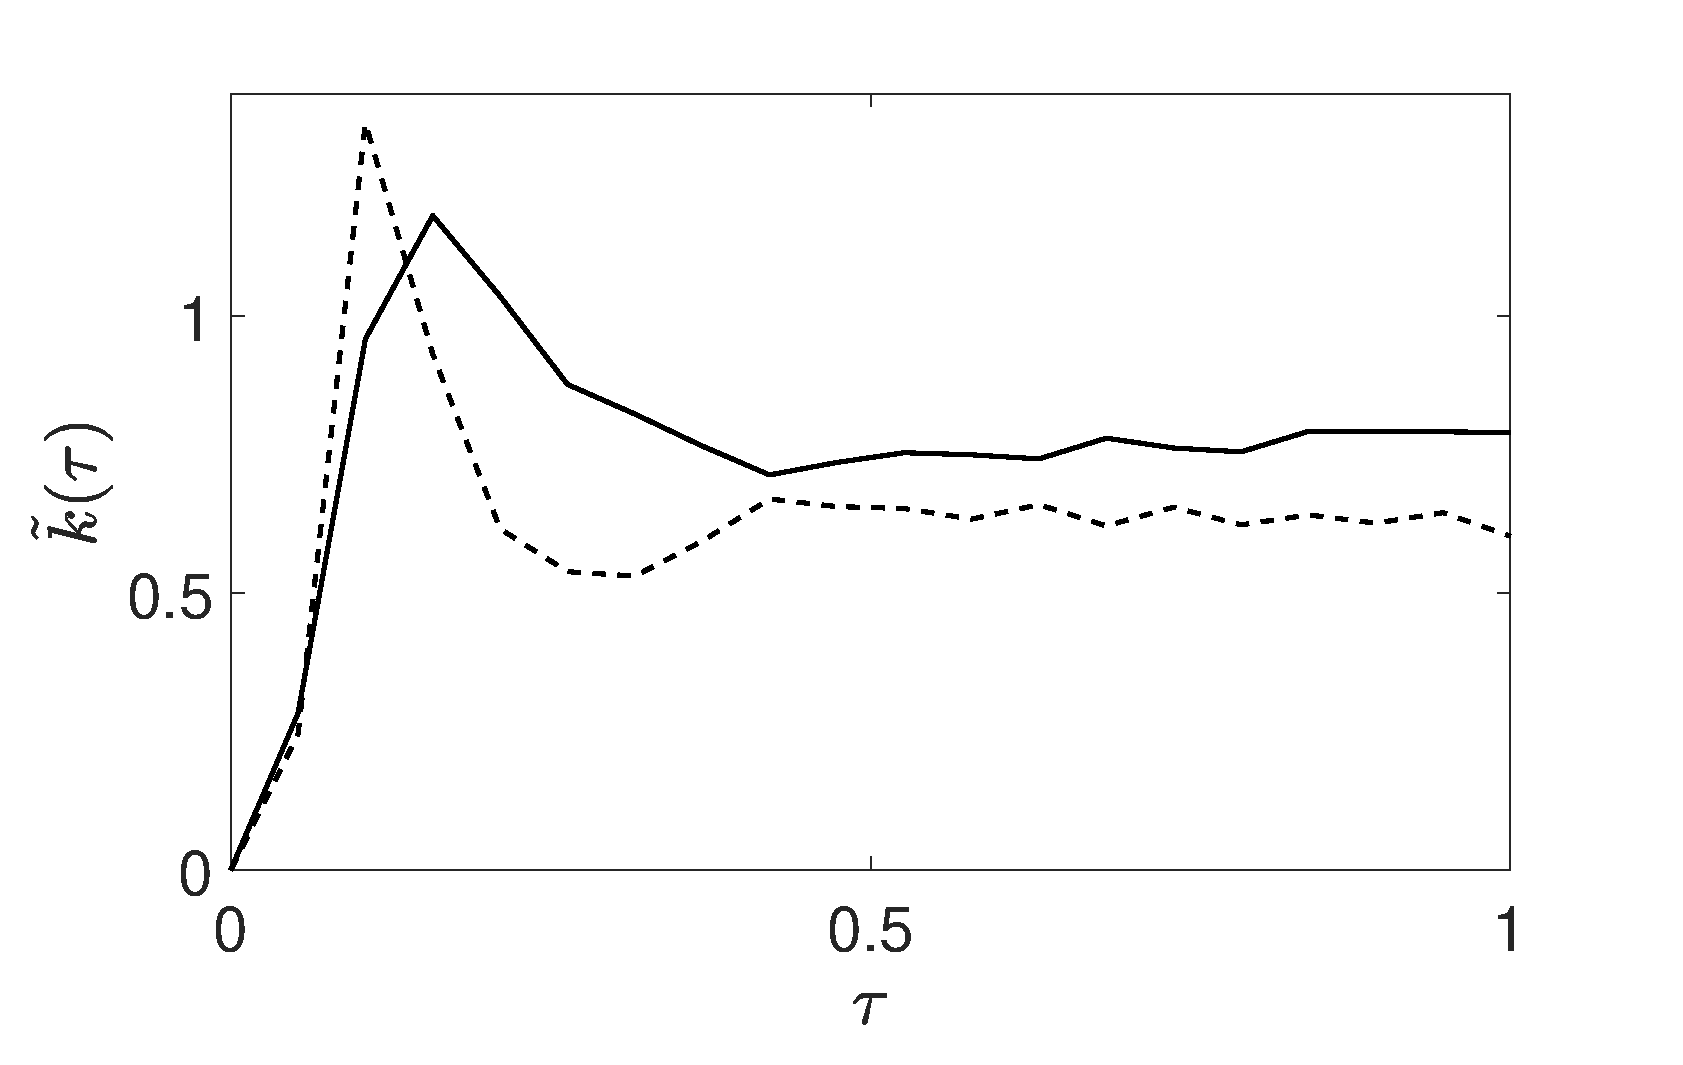
\includegraphics[width=.48\textwidth]{kts_w_nhf_ep_pt05_Nens_512_sig0_1pt05} \\
(c) $\tilde{\sigma}(\tau)$, $\sigma = 1.05\sigma_{c}$ & (d) $\tilde{k}(\tau)$, $\sigma = 1.05\sigma_{c}$\\
\end{tabular}
\caption{For $\omega=-.5$ and $\sigma=1.05 \sigma_{c}$, in (a) the plot of the spectral distribution function $S(k,\tau_{f},1.05\sigma_{c})$, in (b) the plot of the mean $m(\tau)$, in (c) the plot of the standard deviation $\tilde{\sigma}(\tau)$, and in (d) the plot of the kurtosis $\tilde{k}(\tau)$.  In the graphs, the NLSE is (- -), the VDE (-), and the initial distribution is ($\cdots$).}
\label{fig:stbleomnh}
\end{figure}

\begin{figure}[!ht]
\centering
\begin{tabular}{cc}
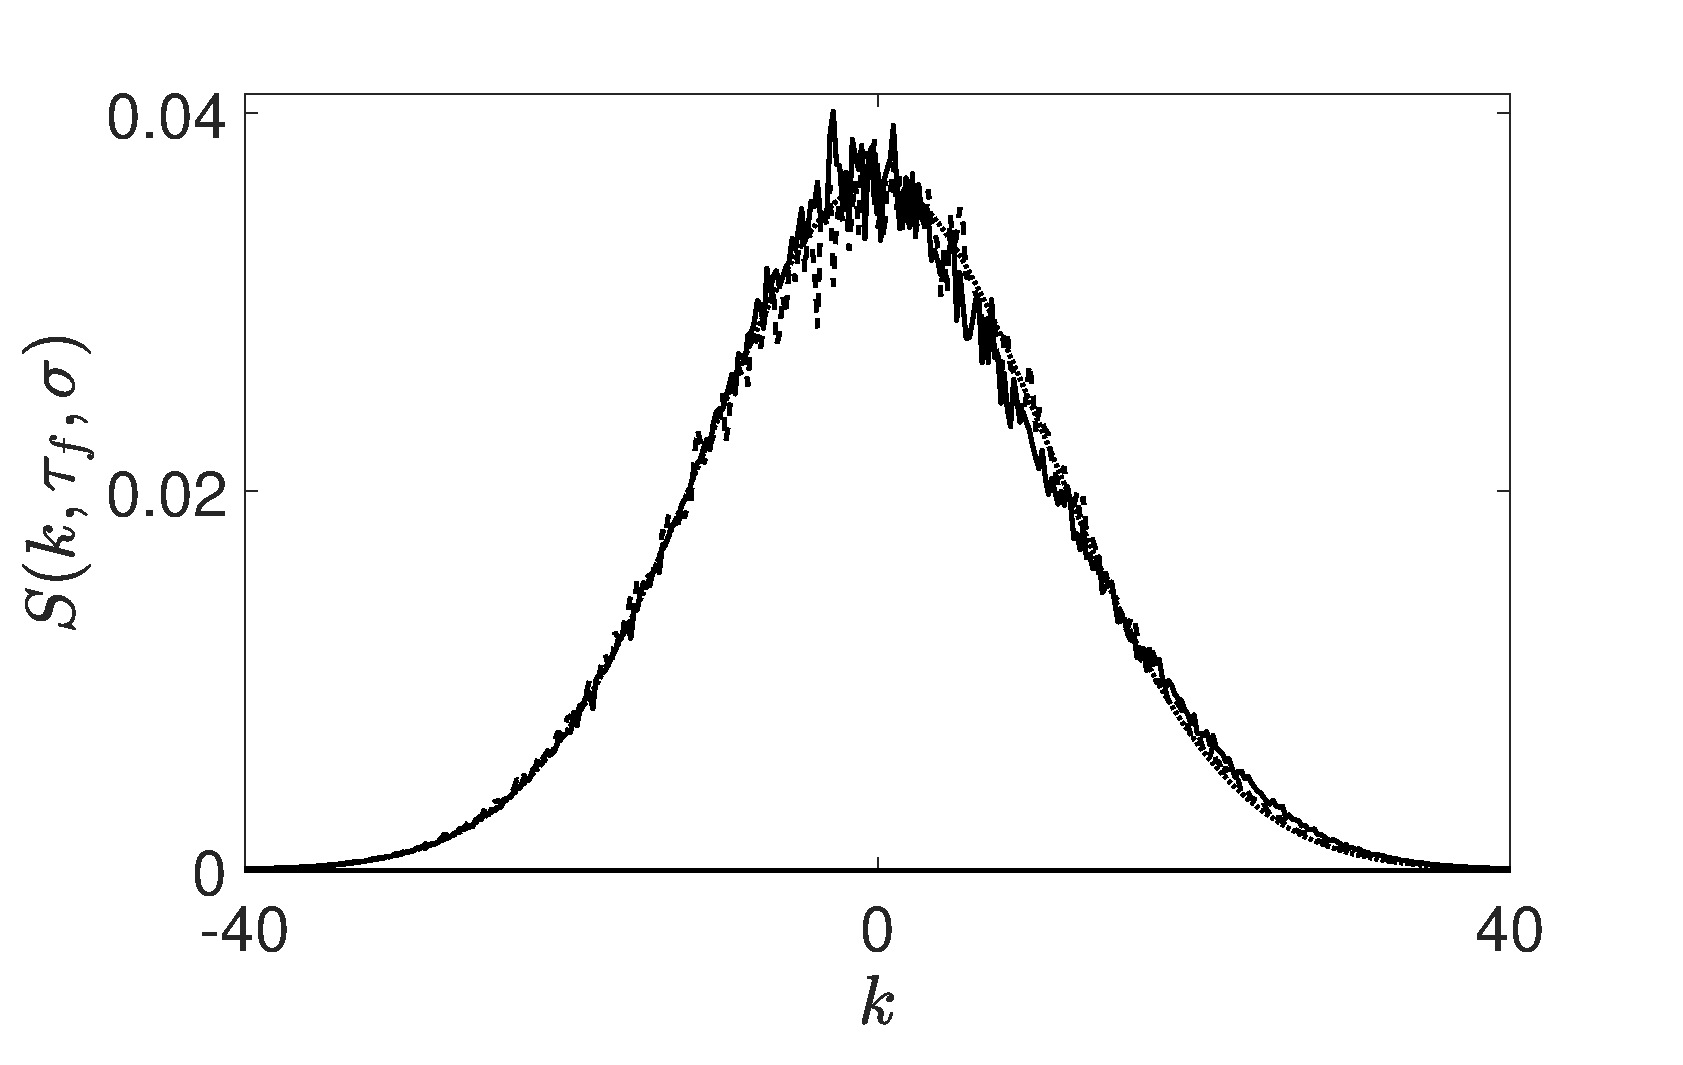
\includegraphics[width=60mm, height=39mm]{pdf_w_nhf_ep_pt05_Nens_512_sig0_2sqrt2} & 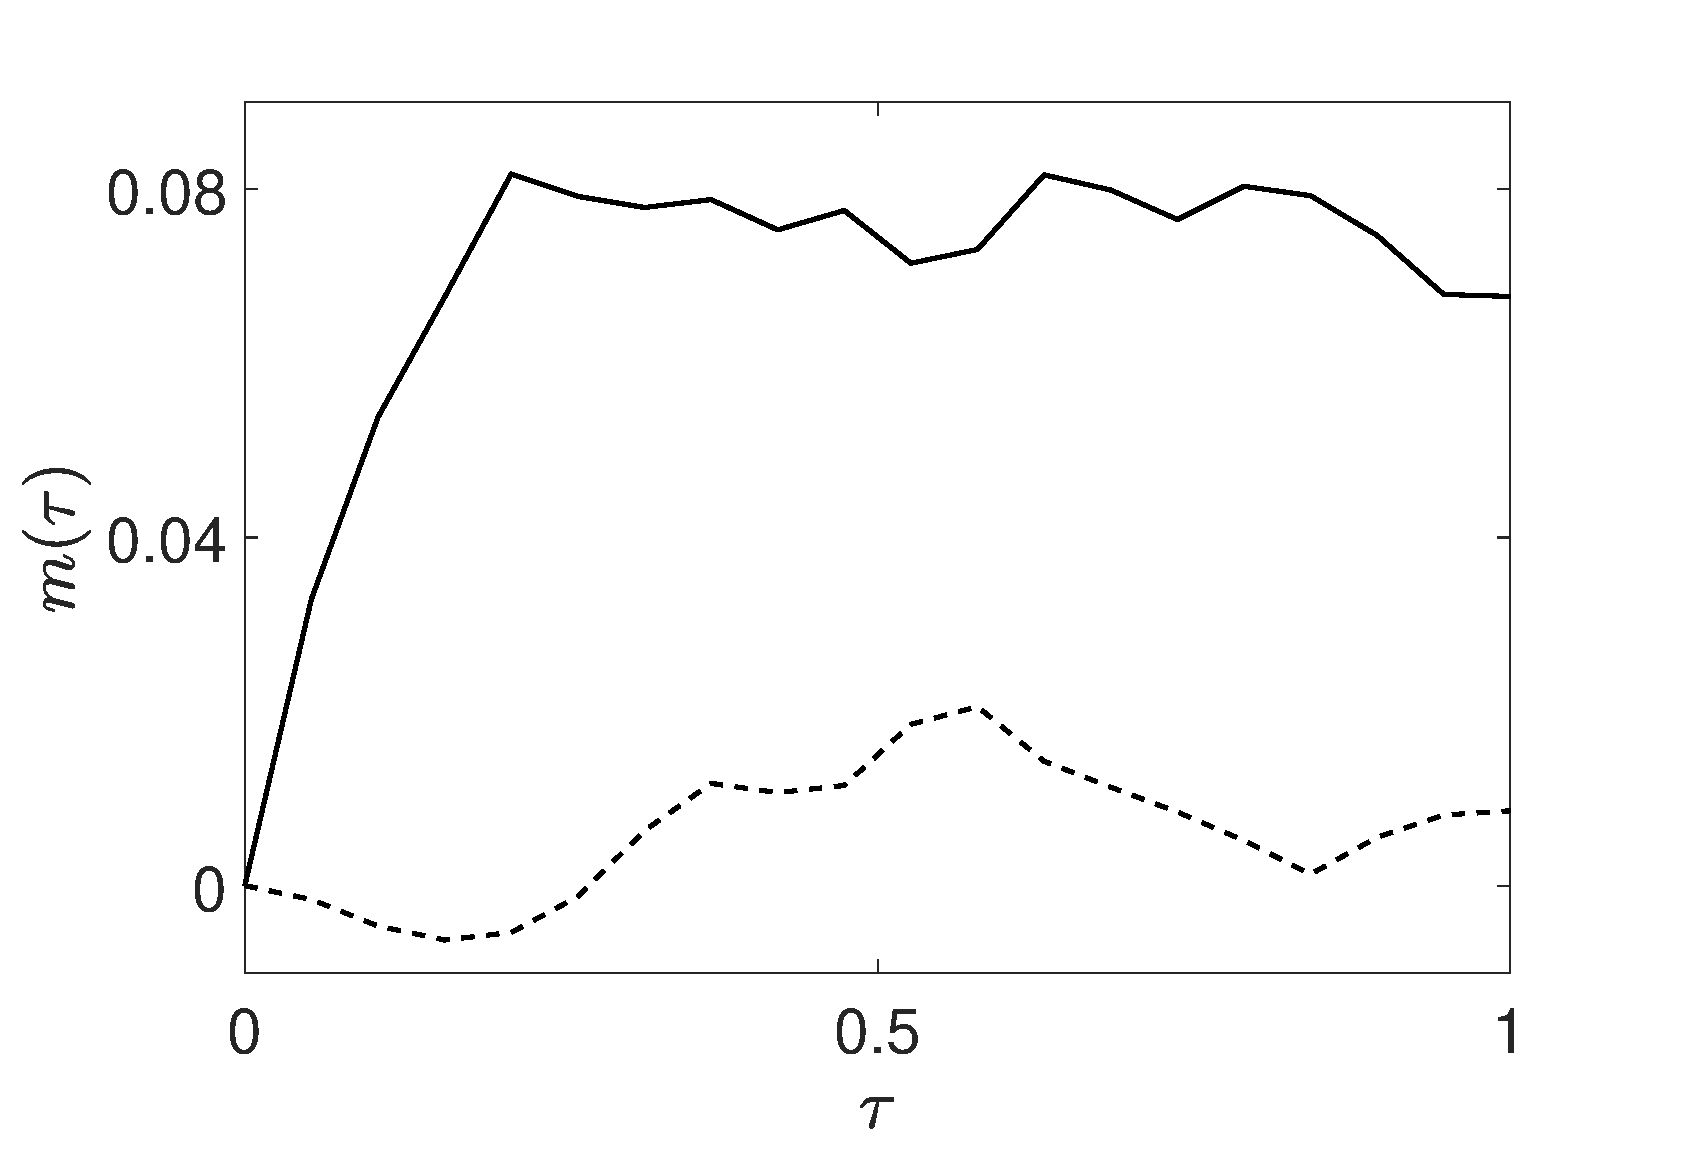
\includegraphics[width=.45\textwidth]{mean_w_nhf_ep_pt05_Nens_512_sig0_2sqrt2} \\
(a) $S(k,\tau_{f},2\sqrt{2}\sigma_{c})$ & (b) $m(\tau)$, $\sigma = 2\sqrt{2}\sigma_{c}$\\
\includegraphics[width=.48\textwidth]{std_w_nhf_ep_pt05_Nens_512_sig0_2sqrt2} & \includegraphics[width=.48\textwidth]{kts_w_nhf_ep_pt05_Nens_512_sig0_2sqrt2} \\
(c) $\tilde{\sigma}(\tau)$, $\sigma = 2\sqrt{2}\sigma_{c}$ & (d) $\tilde{k}(\tau)$, $\sigma = 2\sqrt{2}\sigma_{c}$
\end{tabular}
\caption{For $\omega=-.5$ and $\sigma=2\sqrt{2} \sigma_{c}$, in (a) the plot of the spectral distribution function $S(k,\tau_{f},1.05\sigma_{c})$, in (b) the plot of the mean $m(\tau)$, in (c) the plot of the standard deviation $\tilde{\sigma}(\tau)$, and in (d) the plot of the kurtosis $\tilde{k}(\tau)$.  In the graphs, the NLSE is (- -), the VDE (-), and the initial distribution is ($\cdots$).}
\label{fig:stbleomnhwide}
\end{figure}


\subsection*{Co-Propagating Shear: $\omega = 1.12$}

By letting $\omega=1.12$, corresponding to a shear profile propagating in the direction of the surface wave, we reduce the BFI threshold to $\sigma_{c} \approx 1.01$.  This case becomes the most interesting due to the results in \cite{curtis8} which show that for $k_{0}=1$ that $\omega=1.12$ corresponds to the shear value which most suppresses Stokes drift, i.e. the mean flow of Lagrangian tracers in the fluid.  For this case, the MI timescale is given by $1/\alpha_{nl}\approx 11.8$, so $\tau_{f}\approx 18$.  This far longer time scale is seen in Figure \ref{fig:stbleom1}, where the saturation of the statistics happens just before $\tau_{f}$.  For the narrow initial spectral width $\sigma = 1.05\sigma_{c}$, we see some of the most pronounced deviations between the VDE and NLSE.  As before, there is the inversion in the deviation, see Figure \ref{fig:stbleom1} (c), with the VDE tending to sharpen around the mean.  In this case though, the downshifting in the peak and corresponding one sided skewing of the distribution, see Figure \ref{fig:stbleom1} (a) with its concomitant rise in the kurtosis, \ref{fig:stbleom1} (d), is most dramatic for the $\omega=1.12$ case.  Thus the VDE markedly enhances far-tail phenomena and provides strikingly different predictions than its counterpart model the NLSE.  Thus we see that the the co-propagating shear likely enhances the occurrence of freak wave or other far-tail phenomena for relatively narrow spectral profiles

Of course, as before, when $\sigma=2\sqrt{2}\sigma_{c}$, the added initial spectral width appears to mitigate the impacts of any instabilities or nonlinearity; see Figure \ref{fig:stbleom1wide}.  An interesting point though is that while relatively stable, the widths of the profile for the $\omega=1.12$ case are not as wide as in the previous cases.  This shows that the changed physics coming with the different shear profiles do change the spectral width saturation threshold, and therefore while the BFI condition from \cite{alber} is perhaps incorrect, there clearly is a parameter dependent mechanism which controls the degree to which a given random-wave field achieves a steady statistical state.  
\begin{figure}[!ht]
\centering
\begin{tabular}{cc}
\includegraphics[width=60mm, height=39mm]{pdf_w_1pt12_ep_pt05_Nens_512_sig0_1pt05} & \includegraphics[width=.48\textwidth]{mean_w_1pt12_ep_pt05_Nens_512_sig0_1pt05} \\
(a) $S(k,\tau_{f},1.05\sigma_{c})$ & (b) $m(\tau)$, $\sigma = 1.05\sigma_{c}$\\
\includegraphics[width=.48\textwidth]{std_w_1pt12_ep_pt05_Nens_512_sig0_1pt05} & \includegraphics[width=.48\textwidth]{kts_w_1pt12_ep_pt05_Nens_512_sig0_1pt05} \\
(c) $\tilde{\sigma}(\tau)$, $\sigma = 1.05\sigma_{c}$ & (d) $\tilde{k}(\tau)$, $\sigma = 1.05\sigma_{c}$\\
\end{tabular}
\caption{For $\omega=1.12$ and $\sigma=1.05 \sigma_{c}$, in (a) the plot of the spectral distribution function $S(k,\tau_{f},1.05\sigma_{c})$, in (b) the plot of the mean $m(\tau)$, in (c) the plot of the standard deviation $\tilde{\sigma}(\tau)$, and in (d) the plot of the kurtosis $\tilde{k}(\tau)$.  In the graphs, the NLSE is (- -), the VDE (-), and the initial distribution is ($\cdots$).}
\label{fig:stbleom1}
\end{figure}

\begin{figure}[!ht]
\centering
\begin{tabular}{cc}
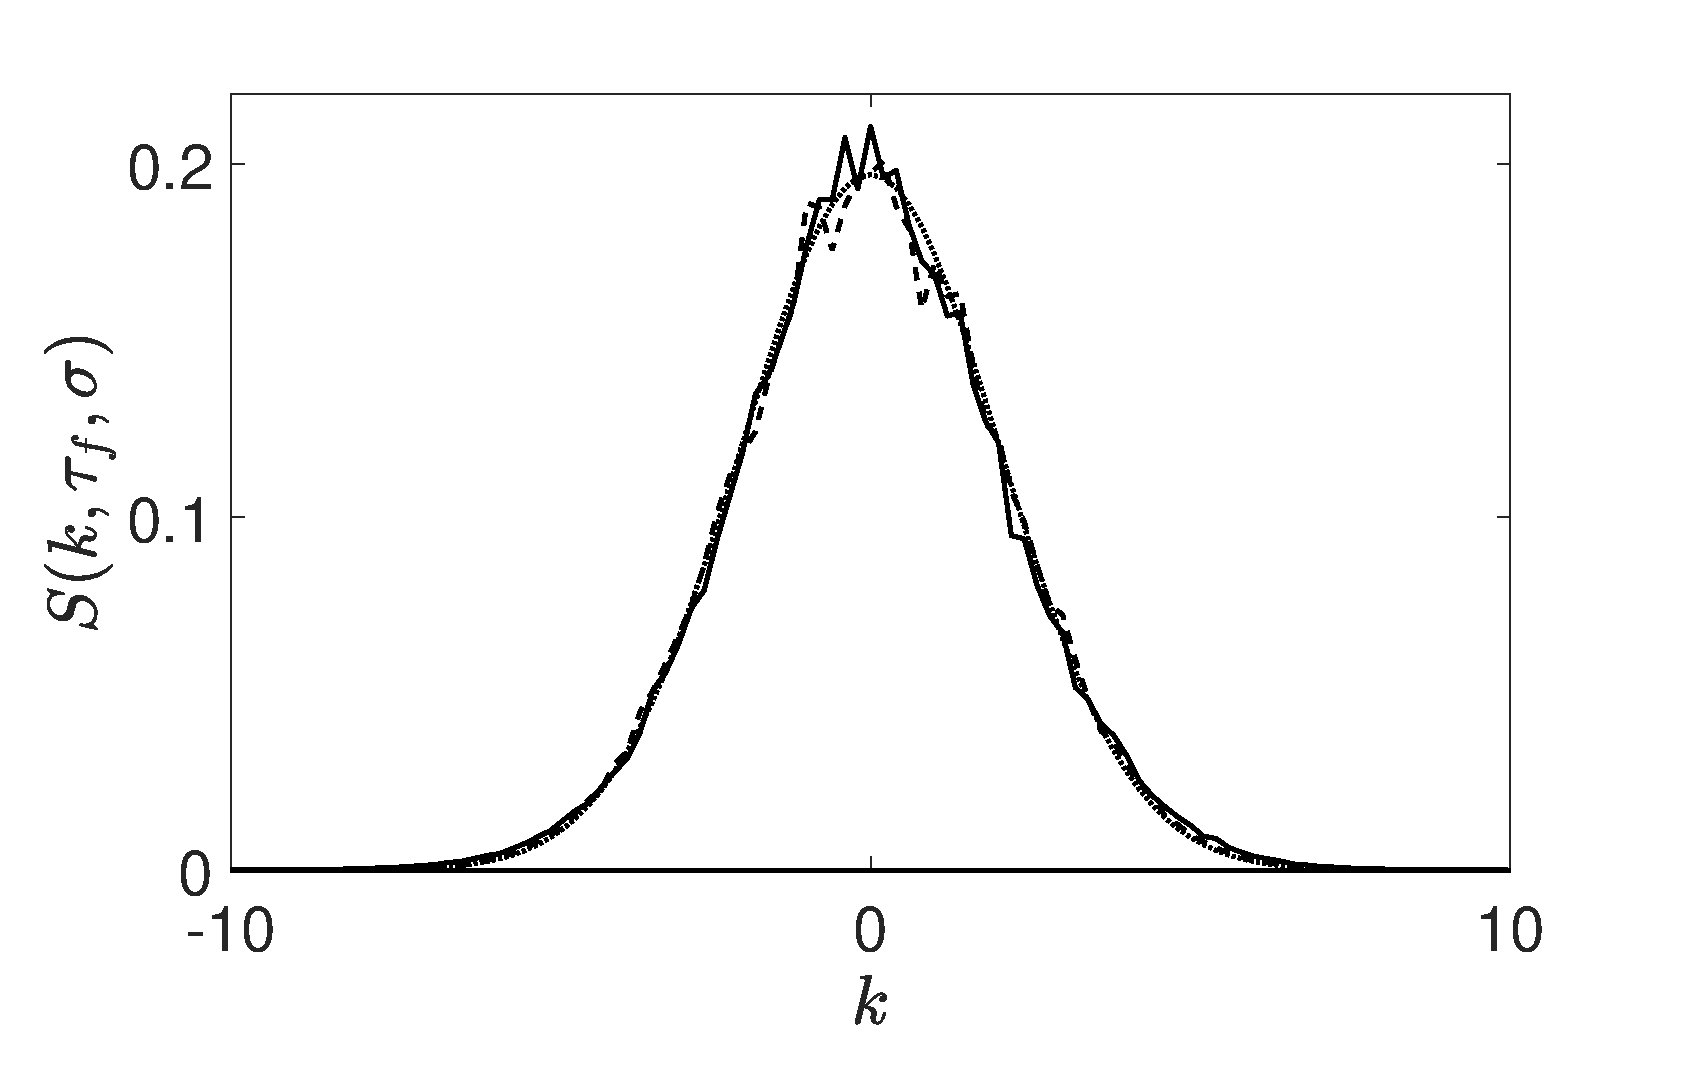
\includegraphics[width=.48\textwidth]{pdf_w_1pt12_ep_pt05_Nens_512_sig0_2sqrt2} & \includegraphics[width=.48\textwidth]{mean_w_1pt12_ep_pt05_Nens_512_sig0_2sqrt2} \\
(a) $S(k,\tau_{f},2\sqrt{2}\sigma_{c})$ & (b) $m(\tau)$, $\sigma = 2\sqrt{2}\sigma_{c}$\\
\includegraphics[width=.48\textwidth]{std_w_1pt12_ep_pt05_Nens_512_sig0_2sqrt2} & \includegraphics[width=.48\textwidth]{kts_w_1pt12_ep_pt05_Nens_512_sig0_2sqrt2} \\
(c) $\tilde{\sigma}(\tau)$, $\sigma = 2\sqrt{2}\sigma_{c}$ & (d) $\tilde{k}(\tau)$, $\sigma = 2\sqrt{2}\sigma_{c}$
\end{tabular}
\caption{For $\omega=1.12$ and $\sigma=2\sqrt{2} \sigma_{c}$, in (a) the plot of the spectral distribution function $S(k,\tau_{f},1.05\sigma_{c})$, in (b) the plot of the mean $m(\tau)$, in (c) the plot of the standard deviation $\tilde{\sigma}(\tau)$, and in (d) the plot of the kurtosis $\tilde{k}(\tau)$.  In the graphs, the NLSE is (- -), the VDE (-), and the initial distribution is ($\cdots$).}
\label{fig:stbleom1wide}
\end{figure}

\subsection*{Kurtosis and the BFI}
Comparing across the plots in Figure \ref{fig:kurtplt}, we summarize the impact that varying BFI indices, or varying initial spectral widths $\sigma$ for $1.05\sigma_{c}\leq \sigma \leq 2\sqrt{2}\sigma_{c}$, have on the kurtosis of the final spectral distributions.  As expected from the plots above, an increasing BFI, or decreasing initial spectral width, corresponds to a stronger kurtosis and thus a stronger deviation away from normality of the final spectral distribution.  Moreover, increasing shear enhances the kurtosis, and finally the higher-order nonlinearities of the VDE always enhance the kurtosis relative to the value predicted by the NLSE.  Likewise, we see that the quadratic fits are clearly good, though also it is clear varying vorticity values change the coefficients of the fit.  This conforms with the results in \cite{eeltink} which show that the quadratic relationship between the kurtosis and the BFI varies depending on different damping and wind profiles.  Thus, varying physics has a significant impact on far-tail phenomena manifesting in real-world situations.  
\begin{figure}[!ht]
\centering
\begin{tabular}{c}
\includegraphics[width=.8\textwidth]{kurtosis_fit_om_0_Nens_128}\\
(a) $\omega = 0$ \\
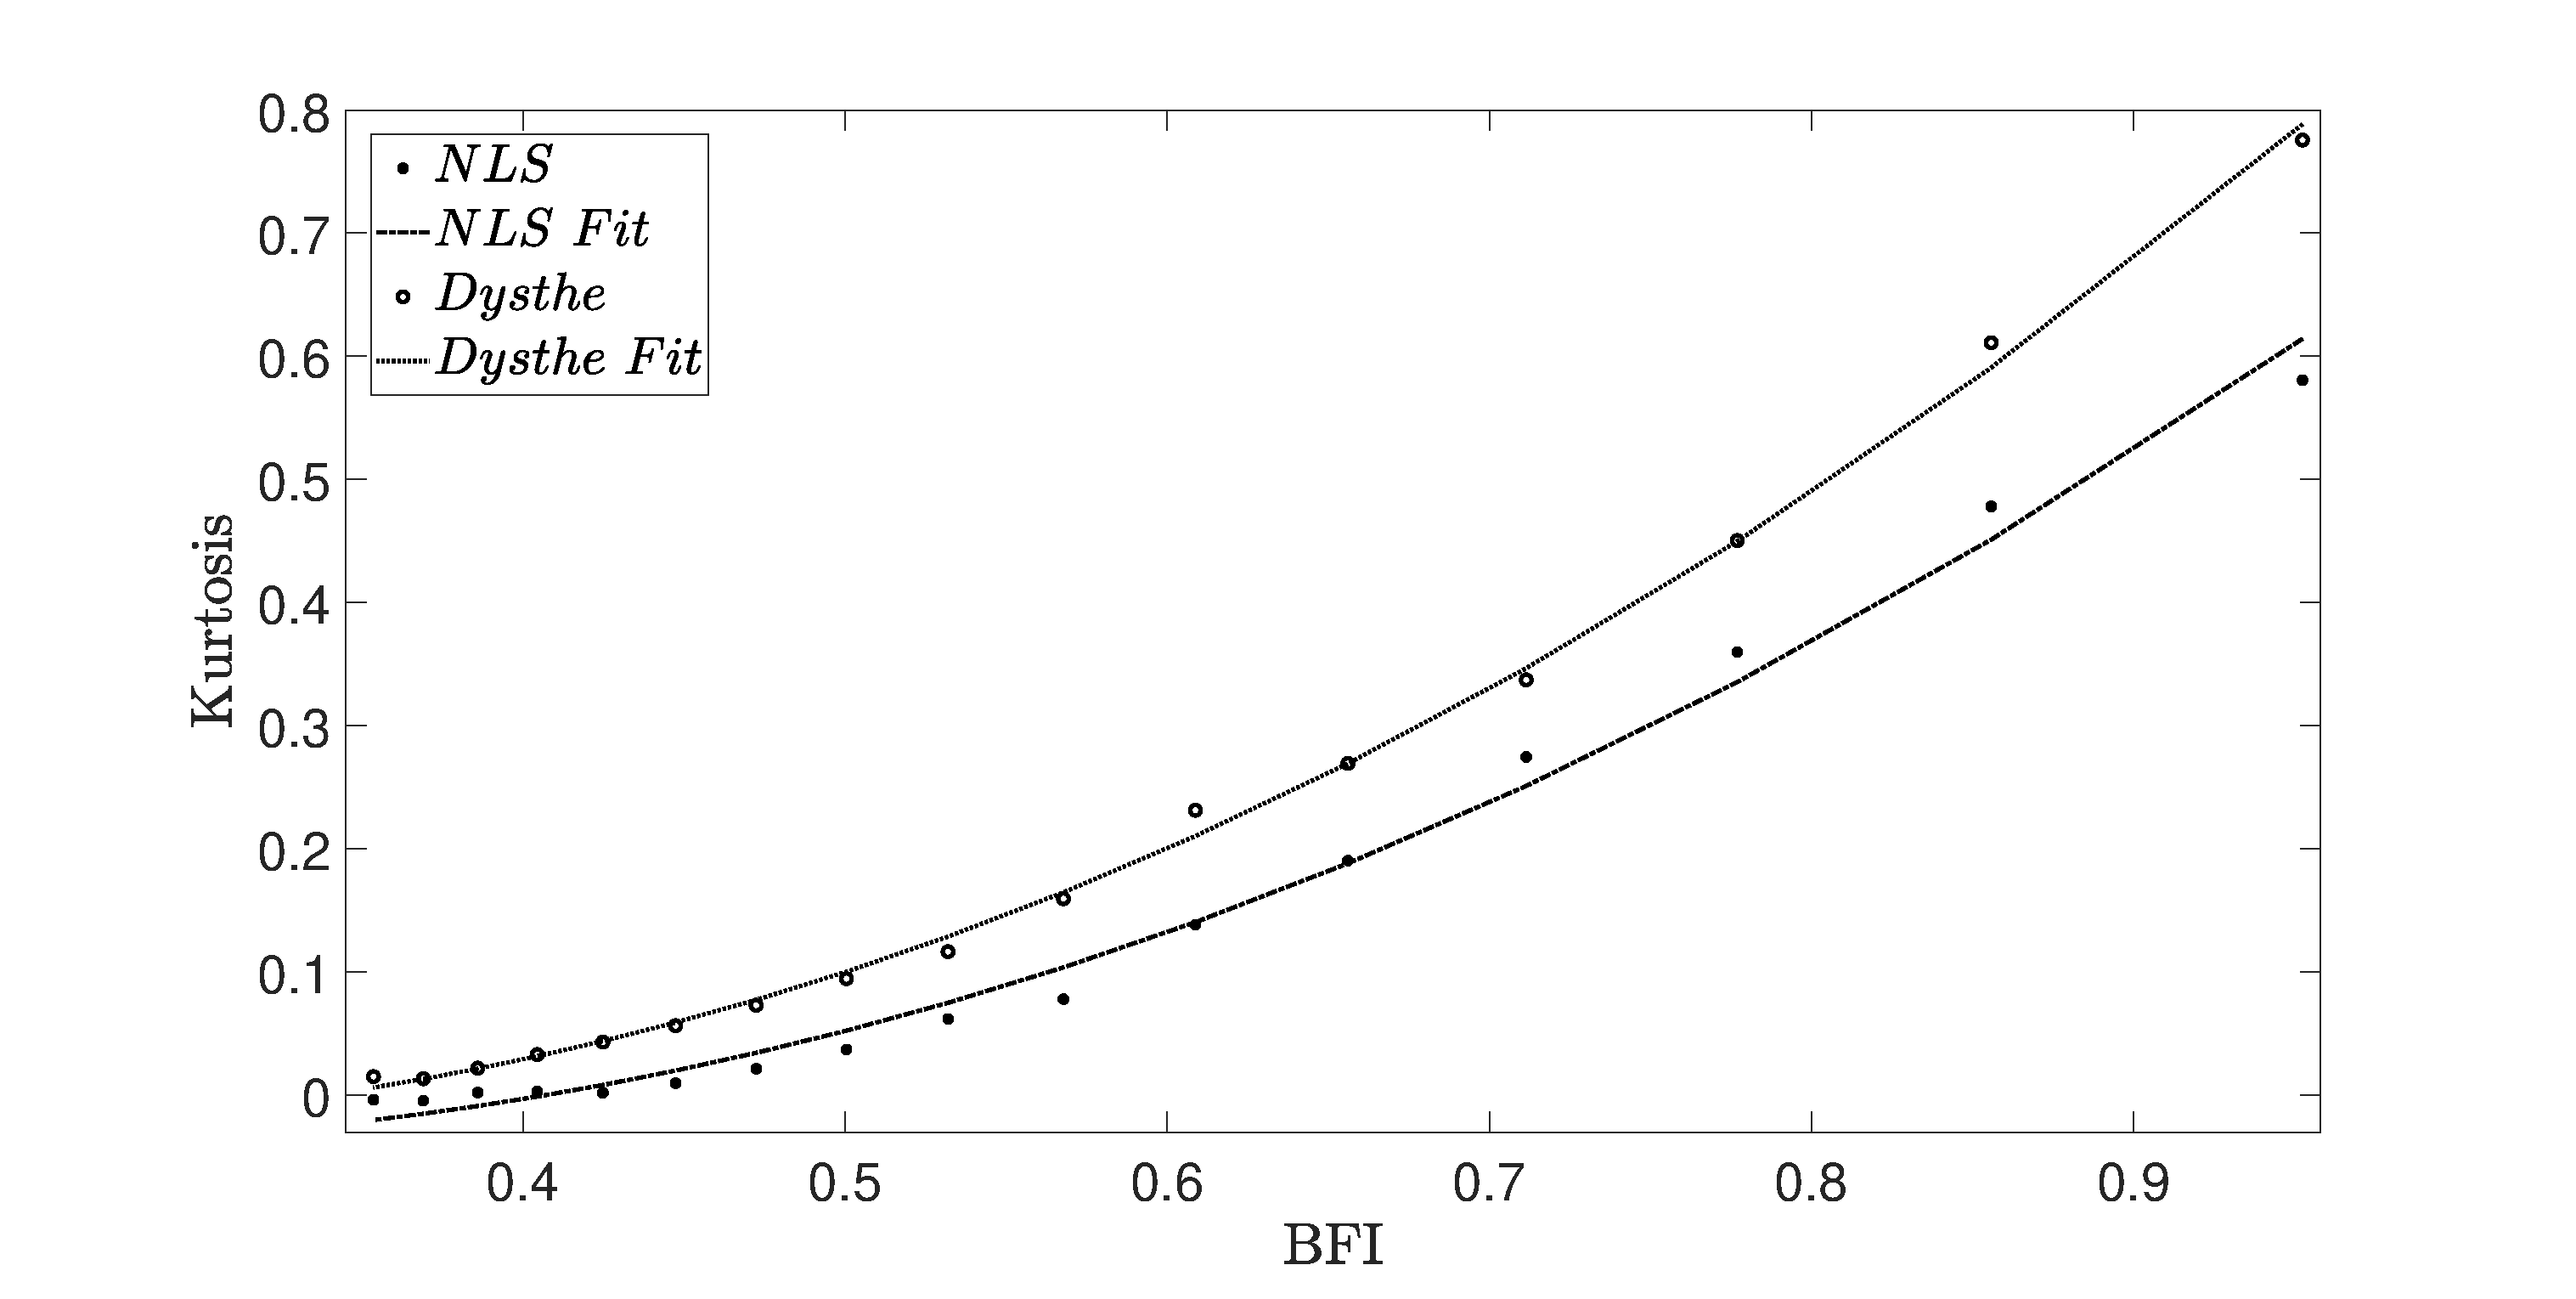
\includegraphics[width=.8\textwidth]{kurtosis_fit_om_nh_Nens_128}\\
(b) $\omega = -.5$\\
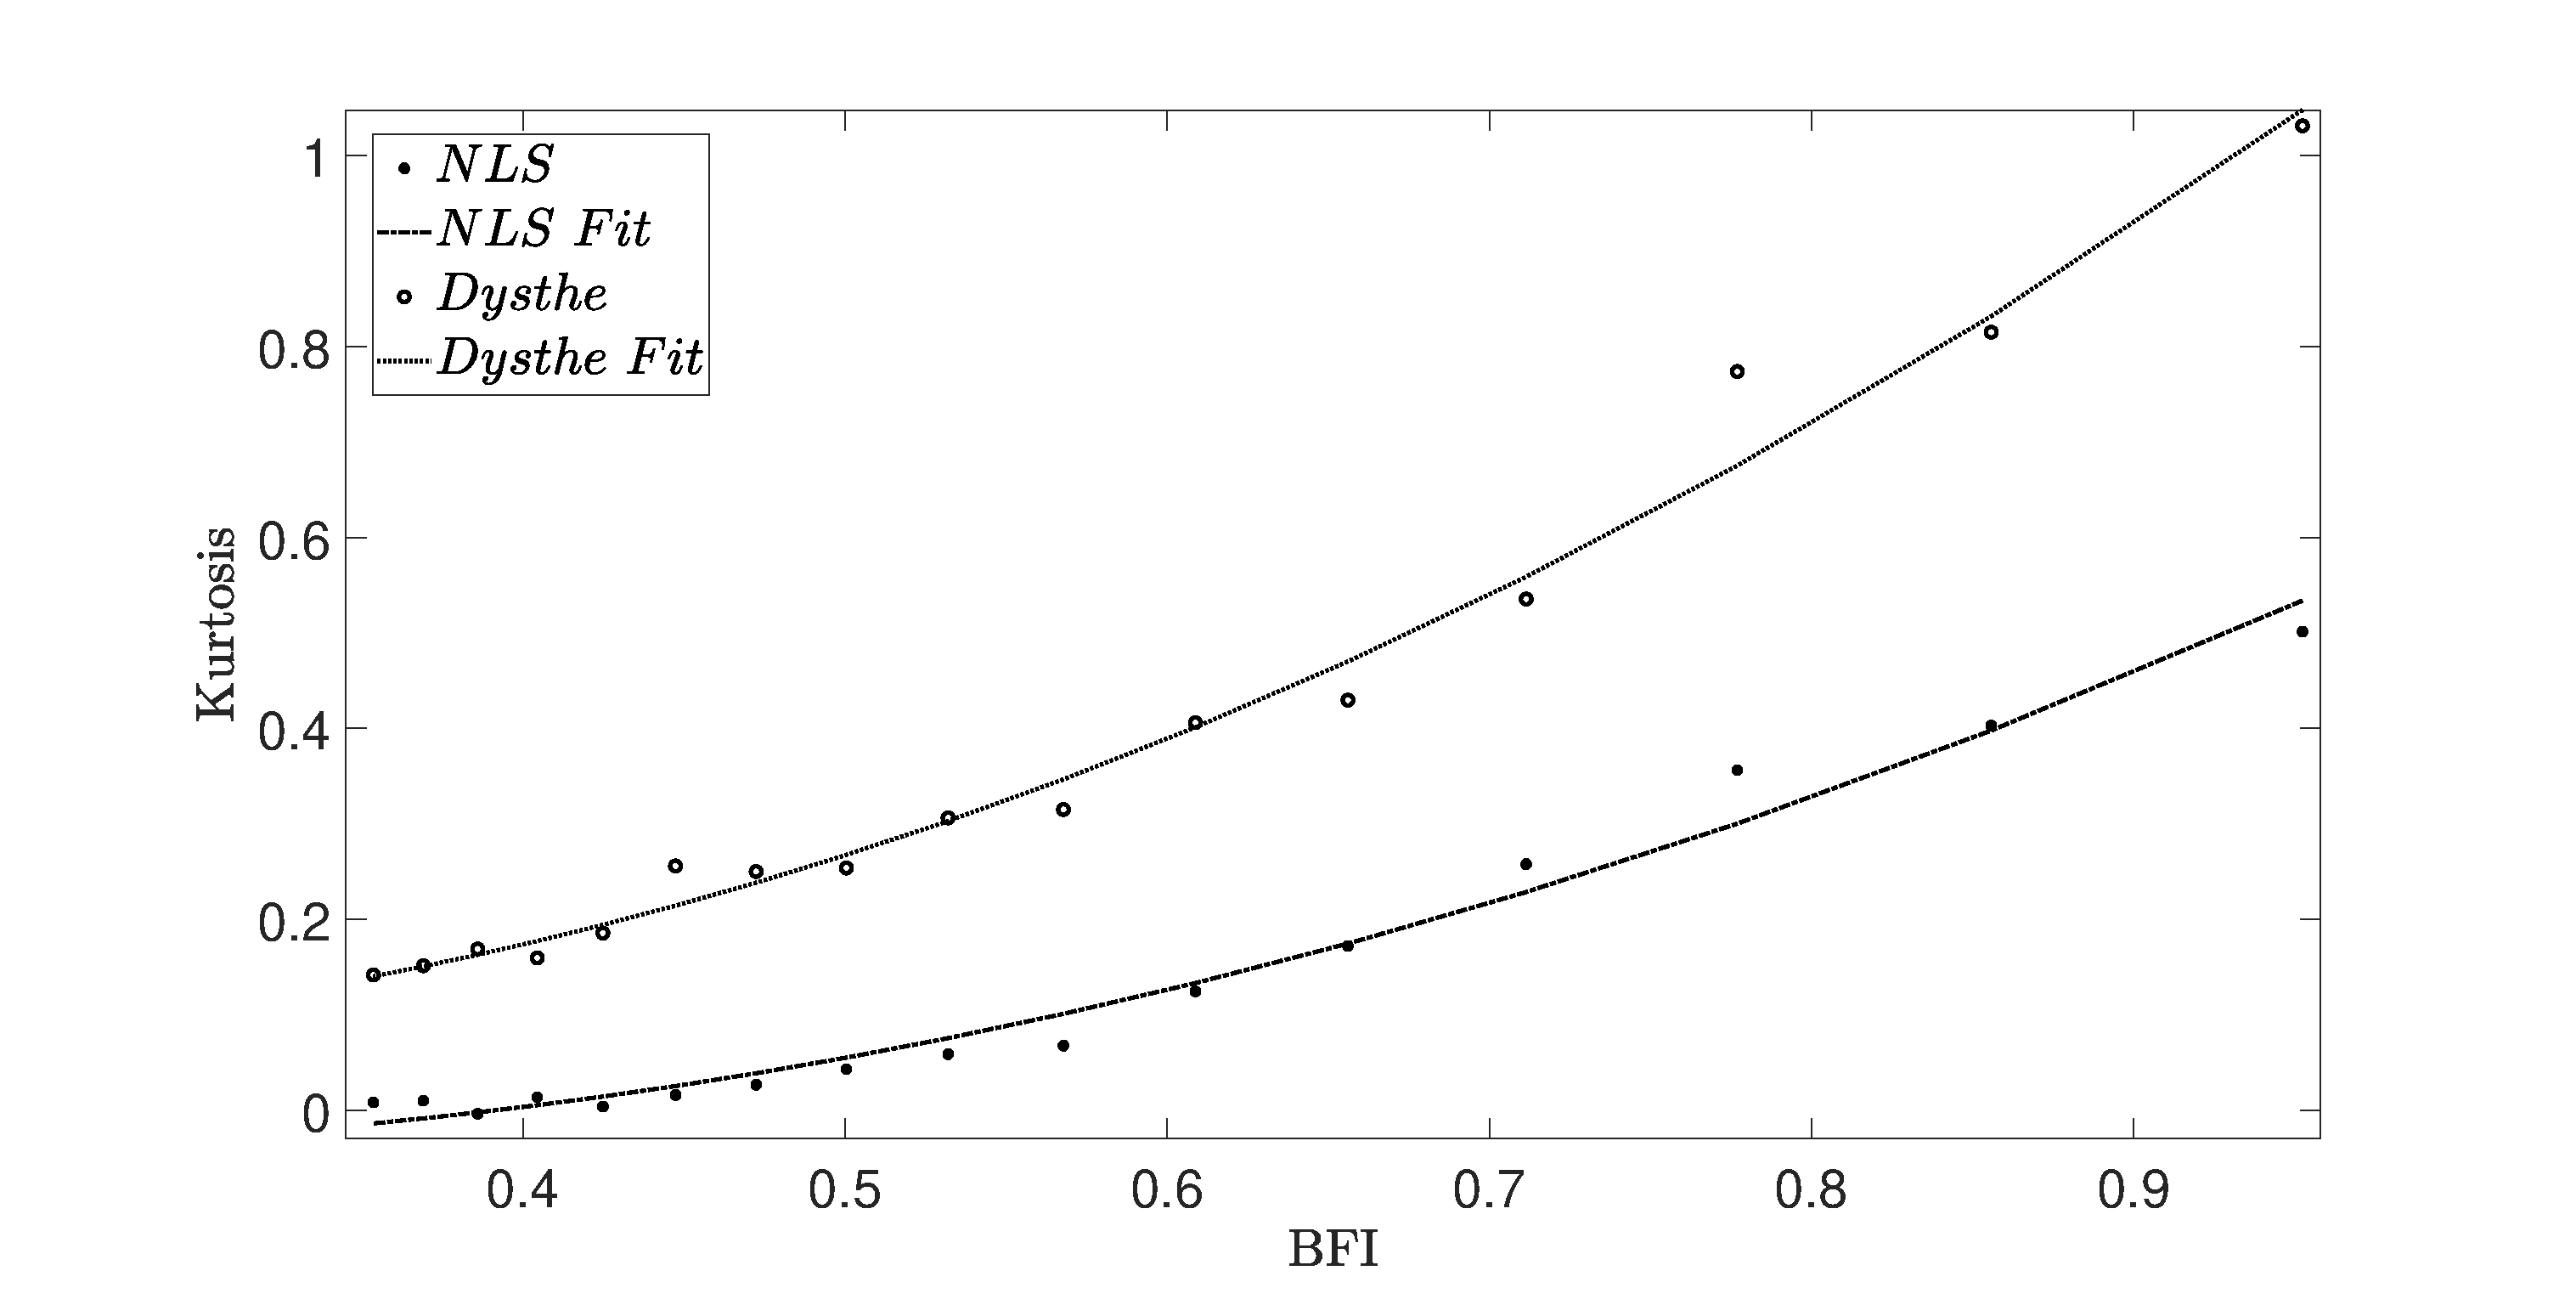
\includegraphics[width=.8\textwidth]{kurtosis_fit_om_1pt12_Nens_128} \\
(c) $\omega=1.12$  
\end{tabular}
\caption{Fixing $\epsilon=.05$, the kurtosis as a function of the BFI for $1.05\sigma_{c}\leq \sigma\leq 2\sqrt{2}\sigma_{c}$ and the corresponding quadratic fits for $\omega=0$ (a), $\omega=-.5$ (b), and $\omega=1.12$ (c).}
\label{fig:kurtplt}
\end{figure}


\section{Conclusion}

In this work, we have studied the impact of modulational stability and other nonlinear effects on the statistical properties of deep-water-surface wave flows moving over constant-vorticity-shear currents.  As we see, the vorticity profile has a strong influence on the stability properties and far tails of the wave train, with co-propagating shears exacerbating modulational instability and higher order nonlinear effects which produce slower decaying tales thereby increasing the likelihood of rare events.  In contrast, counter-propagating shears reduce the impact of modulational instability and higher order nonlinear effects and in turn reduce the likelihood of rare events.  Thus, we see vorticity effects can have significant implications for what the most likely observed deep water wavetrains and phenomena are.  Likewise, in trying to interpret oceanographic data, vortical effects should be taken into account in modeling so as to be able to properly interpret observed data.    

\section*{Acknowledgements}
The authors would like to thank the support of the NSF through DMS-1715039.  Likewise, we appreciate the many conversations and constructive suggestions of John Carter.  On behalf of all authors, the corresponding author states that there is no conflict of interest.

\pagebreak
\bibliography{deep_water_shear_Feb2}
\bibliographystyle{unsrt}
\end{document}